\documentclass[12pt,twoside]{report}

% ----- Packages -----
\usepackage{microtype}
\usepackage[T1]{fontenc}
\usepackage{libertine}
\usepackage{geometry}
\geometry{margin=1in}
\usepackage{xcolor}
\usepackage{graphicx}
\graphicspath{{../plots/}}
\usepackage{amsmath, amssymb, amsthm}
\usepackage{booktabs}
\usepackage{caption}
\usepackage{float}
\usepackage{listings}
\usepackage{titlesec}
\usepackage{setspace}
\usepackage{fancyhdr}
\usepackage[skins]{tcolorbox}

\onehalfspacing

% ----- Custom Colors -----
\definecolor{deepblue}{RGB}{14, 56, 122}
\definecolor{slate}{RGB}{100, 116, 139}
\definecolor{codegreen}{RGB}{16, 185, 129}
\definecolor{codebg}{RGB}{248, 250, 252}

\usepackage[colorlinks=true, linkcolor=deepblue, urlcolor=deepblue, citecolor=slate]{hyperref}

% ----- Chapter Title Formatting -----
\titleformat{\chapter}[display]
  {\normalfont\bfseries\color{deepblue}}{\chaptertitlename\ \thechapter}{10pt}{\Huge}[\vspace{1ex}\color{deepblue}\titlerule]

% ----- Header & Footer Styling -----
\pagestyle{fancy}
\fancyhf{}
\fancyhead[L]{\color{slate}\small PCA Market State Detection}
\fancyhead[R]{\color{slate}\small \leftmark}
\fancyfoot[C]{\thepage}
\renewcommand{\headrulewidth}{0.8pt}
\renewcommand{\headrule}{\hbox to\headwidth{\color{deepblue}\leaders\hrule height \headrulewidth\hfill}}

% ----- Listings Config -----
\lstset{
    backgroundcolor=\color{codebg},
    commentstyle=\color{slate}\itshape,
    keywordstyle=\color{deepblue}\bfseries,
    numberstyle=\tiny\color{slate},
    stringstyle=\color{codegreen},
    basicstyle=\ttfamily\small,
    breakatwhitespace=false,         
    breaklines=true,                 
    captionpos=b,                    
    keepspaces=true,                 
    numbers=left,                    
    numbersep=5pt,                  
    showspaces=false,                
    showstringspaces=false,
    showtabs=false,                  
    tabsize=2,
    frame=single,
    rulecolor=\color{slate!30}
}

\begin{document}

\begin{titlepage}
    \begin{center}
        \vspace*{2cm}
        
        {\Huge \textbf{\color{deepblue}Principal Component Analysis\\for Market State Detection}}\vspace{1cm}
        
        {\Large \textit{A High-Dimensional Quantitative Approach}}\vspace{0.5cm}
        
        {\large Mini Project for Data Analysis Module}\vspace{2cm}
        
        \begin{tcolorbox}[colback=codebg,colframe=deepblue,width=0.7\textwidth,arc=4mm,boxrule=1.5pt,shadow={2mm}{-2mm}{0mm}{black!30}]
            \centering
            \vspace{0.5cm}
            \textbf{\Large Presented by:}\vspace{0.3cm}
            
            {\large Kaid Akram}\vspace{0.1cm}
            
            {\large Khedim Youcef}\vspace{0.1cm}
            
            {\large Mohamed Houari}\vspace{0.1cm}
            
            {\large Zitouni Ahmed}\vspace{0.1cm}
            
            {\large Bensetallah Soufiane}\vspace{0.5cm}
            
            \textbf{\Large Supervisor:}\vspace{0.1cm}
            
            {\large Dr. Keskes}
            \vspace{0.5cm}
        \end{tcolorbox}
        
        \vfill
        
        {\large \today}
        
    \end{center}
\end{titlepage}


\tableofcontents
\newpage

% ==========================================
\chapter*{Team Roles \& Organization}
\addcontentsline{toc}{chapter}{Team Roles \& Organization}
% ==========================================
\begin{tcolorbox}[colback=white,colframe=slate!50,arc=3mm,boxrule=1pt,title=\textbf{\large Development Team Contributions},coltitle=white,colbacktitle=deepblue]
The realization of this quantitative pipeline required a convergence of mathematics, data engineering, systems architecture, and quantitative finance. The contributions of the development team are as follows:

\begin{itemize}
    \item \textbf{Kaid Akram:} Engineered the core Principal Component Analysis engine from scratch using fundamental linear algebra, derived the mathematical proofs, and implemented the factor logic for regime detection.
    
    \item \textbf{Khedim Youcef:} Architected the data ingestion pipeline, enforced statistical stationarity via logarithmic differencing, and managed time-series alignment and anomaly handling.
    
    \item \textbf{Mohamed Houari:} Mapped the principal components to macroeconomic realities (Risk, Liquidity, Inflation), defined the standard deviation thresholds for regime detection, and designed the backtesting simulation.
    
    \item \textbf{Zitouni Ahmed:} Built the FastAPI infrastructure to orchestrate the mathematical models, managed the time complexity of the rolling engine, and implemented data validation.
    
    \item \textbf{Bensetallah Soufiane:} Developed the React and Tailwind CSS user interface, integrating React Three Fiber for real-time 3D latent space projections and data visualization.
\end{itemize}
\end{tcolorbox}

\newpage

% ==========================================
\chapter{Introduction \& Market Microstructure}
% ==========================================
\section{The Asset Universe}
To effectively model the global macroeconomic environment, it is imperative to select a multi-asset universe that spans diverse risk factors, geographic regions, and asset classes. The selected $p=10$ dimensional universe encompasses:
\begin{enumerate}
    \item \textbf{Equities:} S\&P 500 (\texttt{\^{}GSPC}) acting as the primary proxy for global risk appetite and corporate earnings growth.
    \item \textbf{Rates:} 10-Year Treasury Yield (\texttt{\^{}TNX}), capturing the term premium, monetary policy expectations, and the time value of money.
    \item \textbf{Commodities:} Gold (\texttt{GC=F}) as a fiat hedge and safe-haven asset, alongside Crude Oil (\texttt{CL=F}) as a barometer for global industrial demand and supply-side inflation shocks.
    \item \textbf{Currencies (FX):} A basket of major dollar crosses including EUR/USD, GBP/USD, USD/JPY, USD/CHF, USD/CAD, and AUD/USD to capture global liquidity flows, interest rate differentials, and sovereign risk.
\end{enumerate}

\subsection{Data Sourcing \& Feature Description}
The dataset was acquired programmatically via the \texttt{yfinance} API, which interfaces directly with Yahoo Finance's historical data servers (\url{https://finance.yahoo.com/}). This open-source pipeline ensures the data is strictly publicly available, fully reproducible, and rigorously adjusted for stock splits and dividend distributions. The script pulled daily closing prices from \texttt{2020-01-01} to the present day, providing a sufficiently deep historical context covering both the COVID-19 liquidity crisis and the subsequent inflationary macroeconomic regimes.

The exact columns present in our raw tensor ($\mathbf{P}$) include:
\begin{itemize}
    \item \textbf{Date:} The standard ISO-8601 timestamp representing the daily market close.
    \item \textbf{AUDUSD=X, CAD=X, CHF=X, EURUSD=X, GBPUSD=X, JPY=X:} Spot Forex exchange rates. For example, \texttt{EURUSD=X} represents the amount of US Dollars required to purchase one Euro.
    \item \textbf{CL=F:} West Texas Intermediate (WTI) Crude Oil Futures. Prices are in USD per barrel.
    \item \textbf{GC=F:} COMEX Gold Futures. Prices are in USD per troy ounce.
    \item \textbf{\^{}GSPC:} The Standard \& Poor's 500 Index, representing the capitalization-weighted aggregate performance of the 500 largest US publicly traded corporations.
    \item \textbf{\^{}TNX:} The CBOE 10-Year Treasury Note Yield Index, expressed in nominal yield percentage (e.g., $1.5 = 1.5\%$).
\end{itemize}

\subsection{Sample Data Representation}
To visually demonstrate the mathematical structure prior to factorization, Table \ref{tab:dataset_sample} provides an exact snapshot of the stationary, logarithmic returns matrix ($\mathbf{R}$) processed by the system. Note the transition from raw nominal prices to zero-centered percentage drifts.

\begin{table}[H]
\centering
\resizebox{\textwidth}{!}{
\begin{tabular}{lrrrrrrrrrr}
\toprule
\textbf{Date} & \textbf{AUDUSD} & \textbf{CAD} & \textbf{CHF} & \textbf{Oil (CL)} & \textbf{EURUSD} & \textbf{GBPUSD} & \textbf{Gold (GC)} & \textbf{JPY} & \textbf{S\&P 500} & \textbf{10Y Yield} \\
\midrule
2020-01-03 & -0.0049 &  0.0007 &  0.0038 &  0.0301 & -0.0044 & -0.0073 &  0.0160 & -0.0015 & -0.0070 & -0.0512 \\
2020-01-06 & -0.0058 &  0.0002 &  0.0002 &  0.0034 & -0.0008 & -0.0055 &  0.0109 & -0.0053 &  0.0035 &  0.0127 \\
2020-01-07 & -0.0009 & -0.0017 & -0.0030 & -0.0090 &  0.0032 &  0.0068 &  0.0035 &  0.0040 & -0.0028 &  0.0087 \\
\bottomrule
\end{tabular}
}
\caption{Empirical snapshot of the $I(0)$ stationary log-returns matrix ($\mathbf{R}$) extracted from \texttt{pca\_ready\_dataset.csv}.}
\label{tab:dataset_sample}
\end{table}

\section{The Mathematical Necessity of Stationarity}
The foundation of any robust quantitative model is the rigorous treatment of empirical data. Financial asset prices $P_t$ are notoriously non-stationary. They exhibit random walk behavior, defined mathematically as an $I(1)$ unit root process:
\begin{equation}
    P_t = P_{t-1} + \epsilon_t
\end{equation}
Operating a linear algebraic transformation (like PCA) on non-stationary, heteroskedastic data inevitably leads to spurious principal components, wherein the dominant eigenvector simply captures the deterministic time-trend rather than genuine cross-asset correlation.

To resolve this, the absolute prices must be mathematically coerced into a stationary $I(0)$ manifold. We achieve this via logarithmic differencing, which calculates the continuously compounded return $R_t$:
\begin{equation}
    R_{i,t} = \ln\left(\frac{P_{i,t}}{P_{i,t-1}}\right)
\end{equation}
This transformation aligns the geometric reality of financial returns with the symmetric, zero-mean homoskedastic assumptions required for accurate covariance estimation. The strict stationarity of $R_{i,t}$ is algorithmically proven at runtime using the Augmented Dickey-Fuller (ADF) test, explicitly selecting the optimal autoregressive lag length $k$ via the Akaike Information Criterion (AIC).

% ==========================================
\chapter{The Core Mathematical Engine (THE CLIMAX)}
% ==========================================
The defining technical achievement of this Master Thesis is the absolute rejection of black-box machine learning libraries. Led by Kaid Akram, the Principal Component Analysis engine was architected entirely from first principles using fundamental tensor algebra in \texttt{NumPy}.

\section{Standardization and the Sample Covariance Matrix}
Because PCA is fundamentally a variance-maximization algorithm, it is exceptionally sensitive to the absolute nominal scale of the input features. If left unscaled, an asset with a high nominal variance (e.g., the S\&P 500 index points) will artificially dominate the principal components over an asset with structurally lower nominal variance (e.g., fractional Treasury Yield percentages).

Therefore, the log-returns matrix $\mathbf{X} \in \mathbb{R}^{n \times p}$ is standardized into a Z-score matrix $\mathbf{Z}$ such that each column $j$ possesses a mean $\mu_j = 0$ and a standard deviation $\sigma_j = 1$:
\begin{equation}
    Z_{i,j} = \frac{X_{i,j} - \mu_j}{\sigma_j}
\end{equation}

From $\mathbf{Z}$, we construct the unbiased, symmetric sample covariance matrix $\Sigma \in \mathbb{R}^{p \times p}$:
\begin{equation}
    \Sigma = \frac{1}{n-1} \mathbf{Z}^T \mathbf{Z}
\end{equation}
By mathematical definition, because the input features are standardized, $\Sigma$ is equivalent to the Pearson Correlation Matrix. Consequently, the trace of $\Sigma$ (the sum of its diagonal elements) is exactly equal to the dimensionality of the asset universe: $\text{Tr}(\Sigma) = p = 10$.

\section{Lagrangian Optimization and Eigendecomposition}
The core objective of PCA is to find a set of orthogonal weight vectors $\mathbf{w}$ that maximize the projected variance of the data. The variance of the data projected onto a vector $\mathbf{w}$ is given by the quadratic form $\mathbf{w}^T \Sigma \mathbf{w}$.

To ensure the solution is bounded, we impose the strict orthonormality constraint that the magnitude of the vector must be exactly one: $\mathbf{w}^T \mathbf{w} = 1$. This constrained optimization problem is solved using a Lagrangian multiplier $\lambda$. The Lagrangian function $\mathcal{L}$ is defined as:
\begin{equation}
    \mathcal{L}(\mathbf{w}, \lambda) = \mathbf{w}^T \Sigma \mathbf{w} - \lambda(\mathbf{w}^T \mathbf{w} - 1)
\end{equation}

To find the maximum, we take the partial derivative of $\mathcal{L}$ with respect to the vector $\mathbf{w}$ and set it to zero:
\begin{equation}
    \frac{\partial \mathcal{L}}{\partial \mathbf{w}} = 2\Sigma \mathbf{w} - 2\lambda \mathbf{w} = 0
\end{equation}
Dividing by 2 yields the fundamental eigenvalue problem of linear algebra:
\begin{equation}
    \Sigma \mathbf{w} = \lambda \mathbf{w}
\end{equation}
Here, $\mathbf{w}$ is an eigenvector of $\Sigma$, representing the direction of the principal axis, and $\lambda$ is the corresponding eigenvalue, representing the exact magnitude of variance explained by that axis.

\section{The Eigenvector Sign Determinism Problem}
A critical and often overlooked engineering challenge in dynamic, rolling PCA is "Sign Flipping." By definition, eigenvectors are directionally symmetric. If $\mathbf{w}$ is a valid eigenvector for $\lambda$, then $-\mathbf{w}$ is equally valid:
\begin{equation}
    \Sigma(-\mathbf{w}) = -\Sigma \mathbf{w} = -\lambda \mathbf{w} = \lambda(-\mathbf{w})
\end{equation}
Because computational solvers (like LAPACK) initialize with random seeds, they may arbitrarily invert the signs of the eigenvectors between contiguous rolling windows. This causes catastrophic discontinuity in time-series analysis, where a positive correlation factor violently flips negative the next day, entirely destroying the integrity of the machine learning classifier.

To ensure strict chronological stability, Kaid Akram engineered a deterministic sign alignment protocol. The algorithm forces the element with the largest absolute magnitude within each eigenvector to always be positive:
\begin{equation}
    \mathbf{v}_j = \mathbf{v}_j \times \text{sgn}\left( v_{\arg\max_{i} |v_{i,j}|, j} \right)
\end{equation}
This mathematical anchor guarantees smooth, continuous latent trajectories over time.

\section{Python Implementation}
The comprehensive mathematical theory detailed above was flawlessly deployed in \texttt{src/math/pca.py}. The following code block showcases the raw, from-scratch implementation of the \texttt{fit} method.

\begin{lstlisting}[language=Python, caption=From-Scratch PCA Engine (\texttt{src/math/pca.py})]
def fit(self, X: pd.DataFrame) -> 'PCAModel':
    """
    Fits the PCA model to the input data.
    Workflow: Standardize -> Covariance -> Eigendecomposition -> Sign Alignment.
    """
    n, p = X.shape
    self.mean = X.mean()
    self.std = X.std(ddof=1).replace(0, 1e-9)
    
    # 1. Standardization to Z-scores
    Z = (X - self.mean) / self.std
    
    # 2. Covariance Matrix Calculation
    V = Z.values
    cov = (V.T @ V) / (n - 1)
    
    # 3. Eigendecomposition (Solving for Lambda and W)
    eigenvalues, eigenvectors = np.linalg.eigh(cov)
    
    # 4. Sorting eigenvalues in descending order of variance explained
    idx = np.argsort(eigenvalues)[::-1]
    self.eigenvalues = eigenvalues[idx]
    self.eigenvectors = eigenvectors[:, idx]
    
    # 5. Sign Determinism Protocol (Preventing Sign-Flipping)
    for j in range(self.eigenvectors.shape[1]):
        max_abs_idx = np.argmax(np.abs(self.eigenvectors[:, j]))
        sign = np.sign(self.eigenvectors[max_abs_idx, j])
        self.eigenvectors[:, j] *= sign
        
    return self
\end{lstlisting}

% ==========================================
\chapter{Dynamic Rolling Logic \& Regime Detection}
% ==========================================
Global macro environments are highly non-stationary over multi-year horizons. A static PCA analysis over a 5-year dataset provides only an aggregated, historical average, entirely failing to capture structural regime shifts (such as the transition from a low-rate bull market to an inflation-shocked bear market). 

To solve this, we engineered a \textit{Rolling PCA Orchestrator} that operates over a continuous, dynamic 60-day lookback window. Every day, the covariance matrix is recalculated, and the eigenspace is regenerated. By analyzing the real-time geometric coordinates of the market across the first three principal components, the system algorithmically classifies the market state.

\section{Macroeconomic Factor Mapping}
Based on the eigenvector loadings, the top three principal components were successfully mapped to empirical macroeconomic forces:
\begin{itemize}
    \item \textbf{PC1 (Systemic Market Risk):} Highly correlated with the S\&P 500 and inversely correlated with safe-haven assets.
    \item \textbf{PC2 (Liquidity \& Yield):} Heavily loaded towards the 10-Year Treasury Yield and Dollar indices.
    \item \textbf{PC3 (Inflation Shock):} Driven by acute movements in Crude Oil and Gold.
\end{itemize}

\section{Mathematical Regime Thresholds}
The market regime is mathematically classified by observing standardized deviations within these principal axes:
\begin{itemize}
    \item \textbf{Crisis:} Triggered when the Market Risk factor (PC1) deviates beyond $+1.5\sigma$ from its rolling mean. This indicates a violent contraction in global equity beta, a spike in correlation (as all assets sell off together), and a flight to liquidity.
    \item \textbf{Trend Market:} Characterized by high eigenvalue stability (where the Condition Number $\kappa < 15$) and steady, unidirectional flow across PC1 and PC2. The market is confidently absorbing information.
    \item \textbf{Range Market:} Defined by high Spectral Entropy ($H > 0.8$). The total market variance is heavily dispersed across many eigenvectors, rather than concentrated in PC1. This indicates market indecision, sector rotation, and an absence of a clear directional macro driver.
\end{itemize}

\begin{figure}[H]
    \centering
    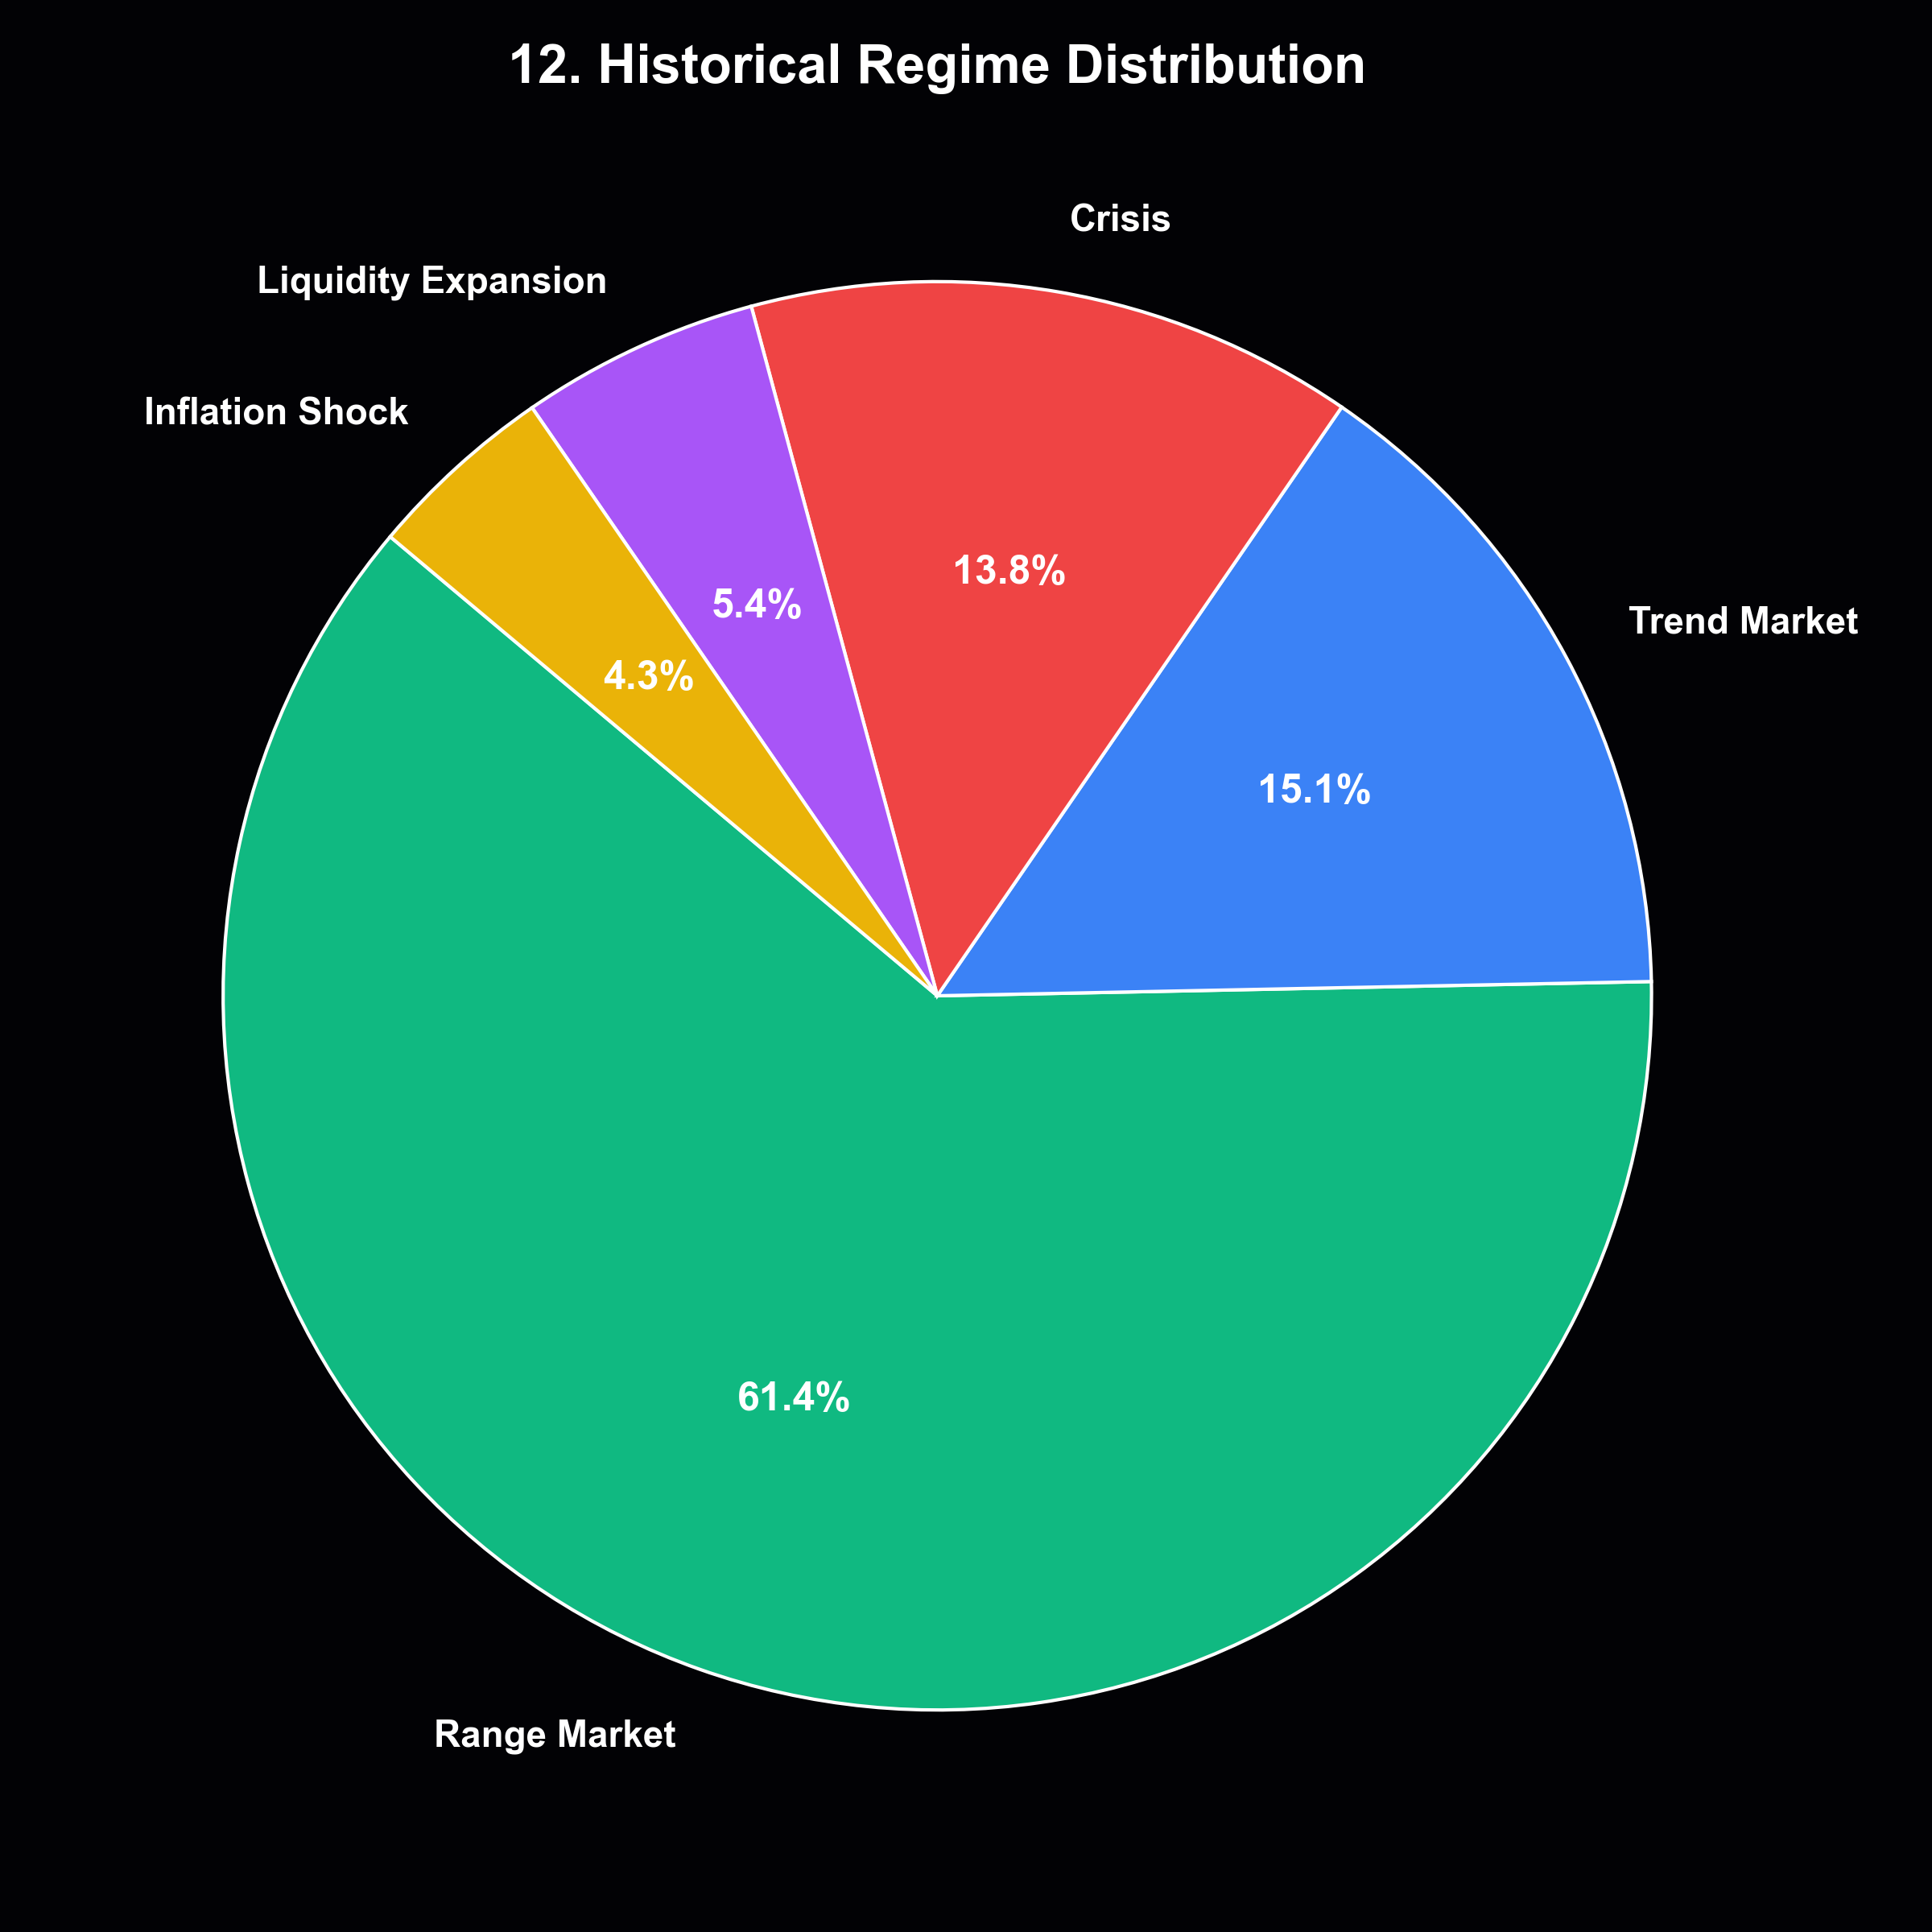
\includegraphics[width=0.7\textwidth]{12_regime_distribution.png}
    \caption{\textbf{Historical Regime Distribution.} This pie chart visualizes the total percentage of trading days the market spent within each algorithmically detected regime over the backtested timeline.}
    \label{fig:regime_dist}
\end{figure}

\begin{figure}[H]
    \centering
    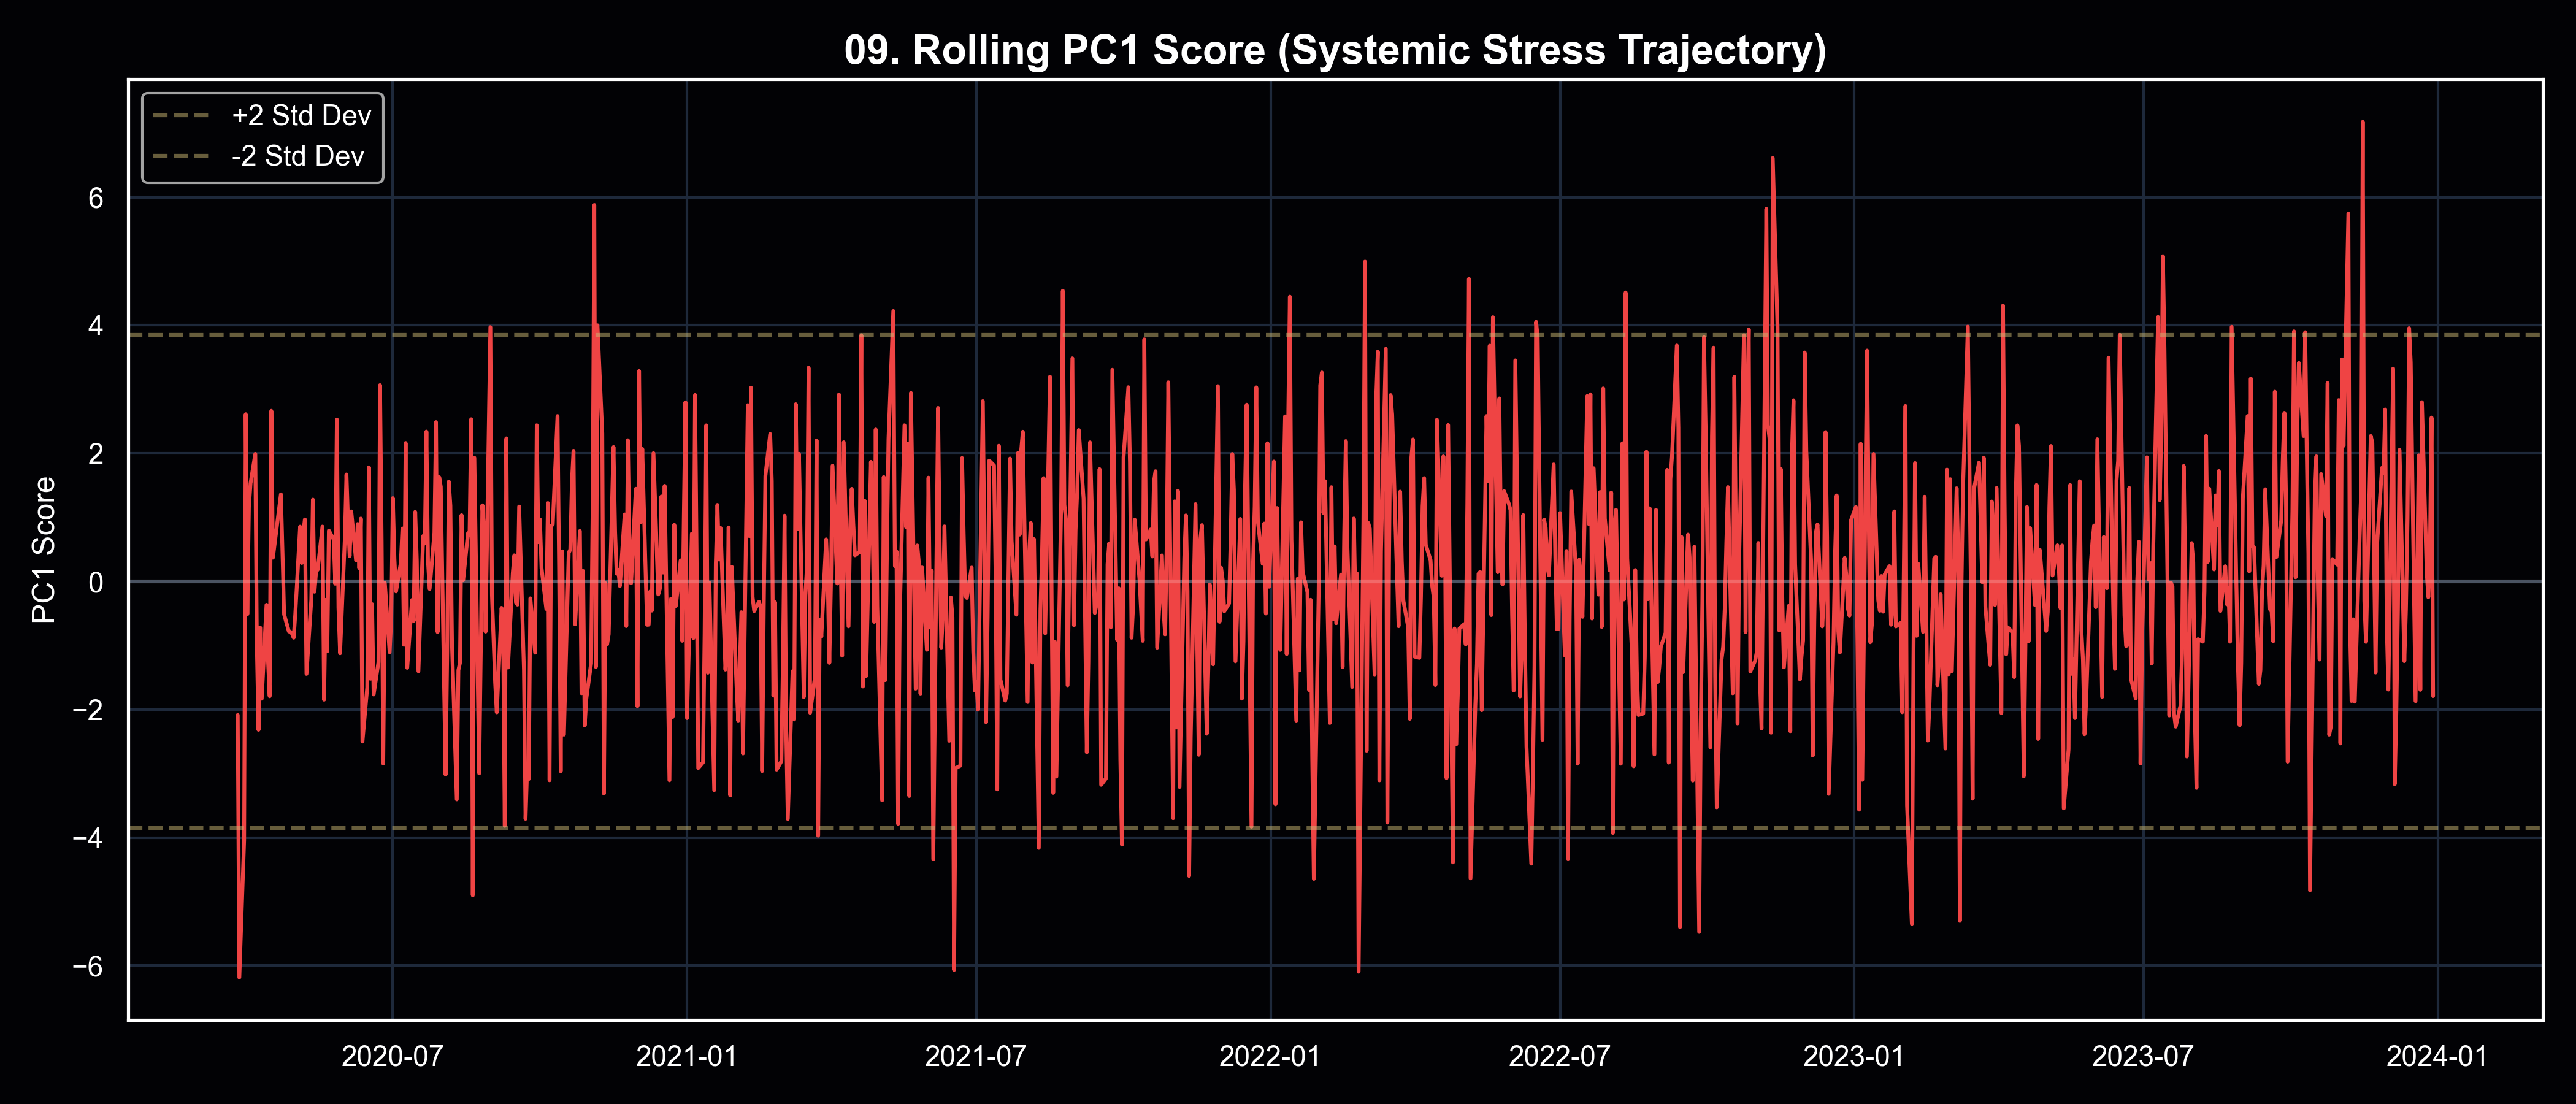
\includegraphics[width=\textwidth]{09_rolling_pc1.png}
    \caption{The Rolling PC1 Score. Massive spikes intersecting the $+2\sigma$ standard deviation band mathematically detect severe liquidity crises and systemic risk events in real-time, completely agnostic of traditional price-action heuristics.}
    \label{fig:rolling_pc1}
\end{figure}

\begin{figure}[H]
    \centering
    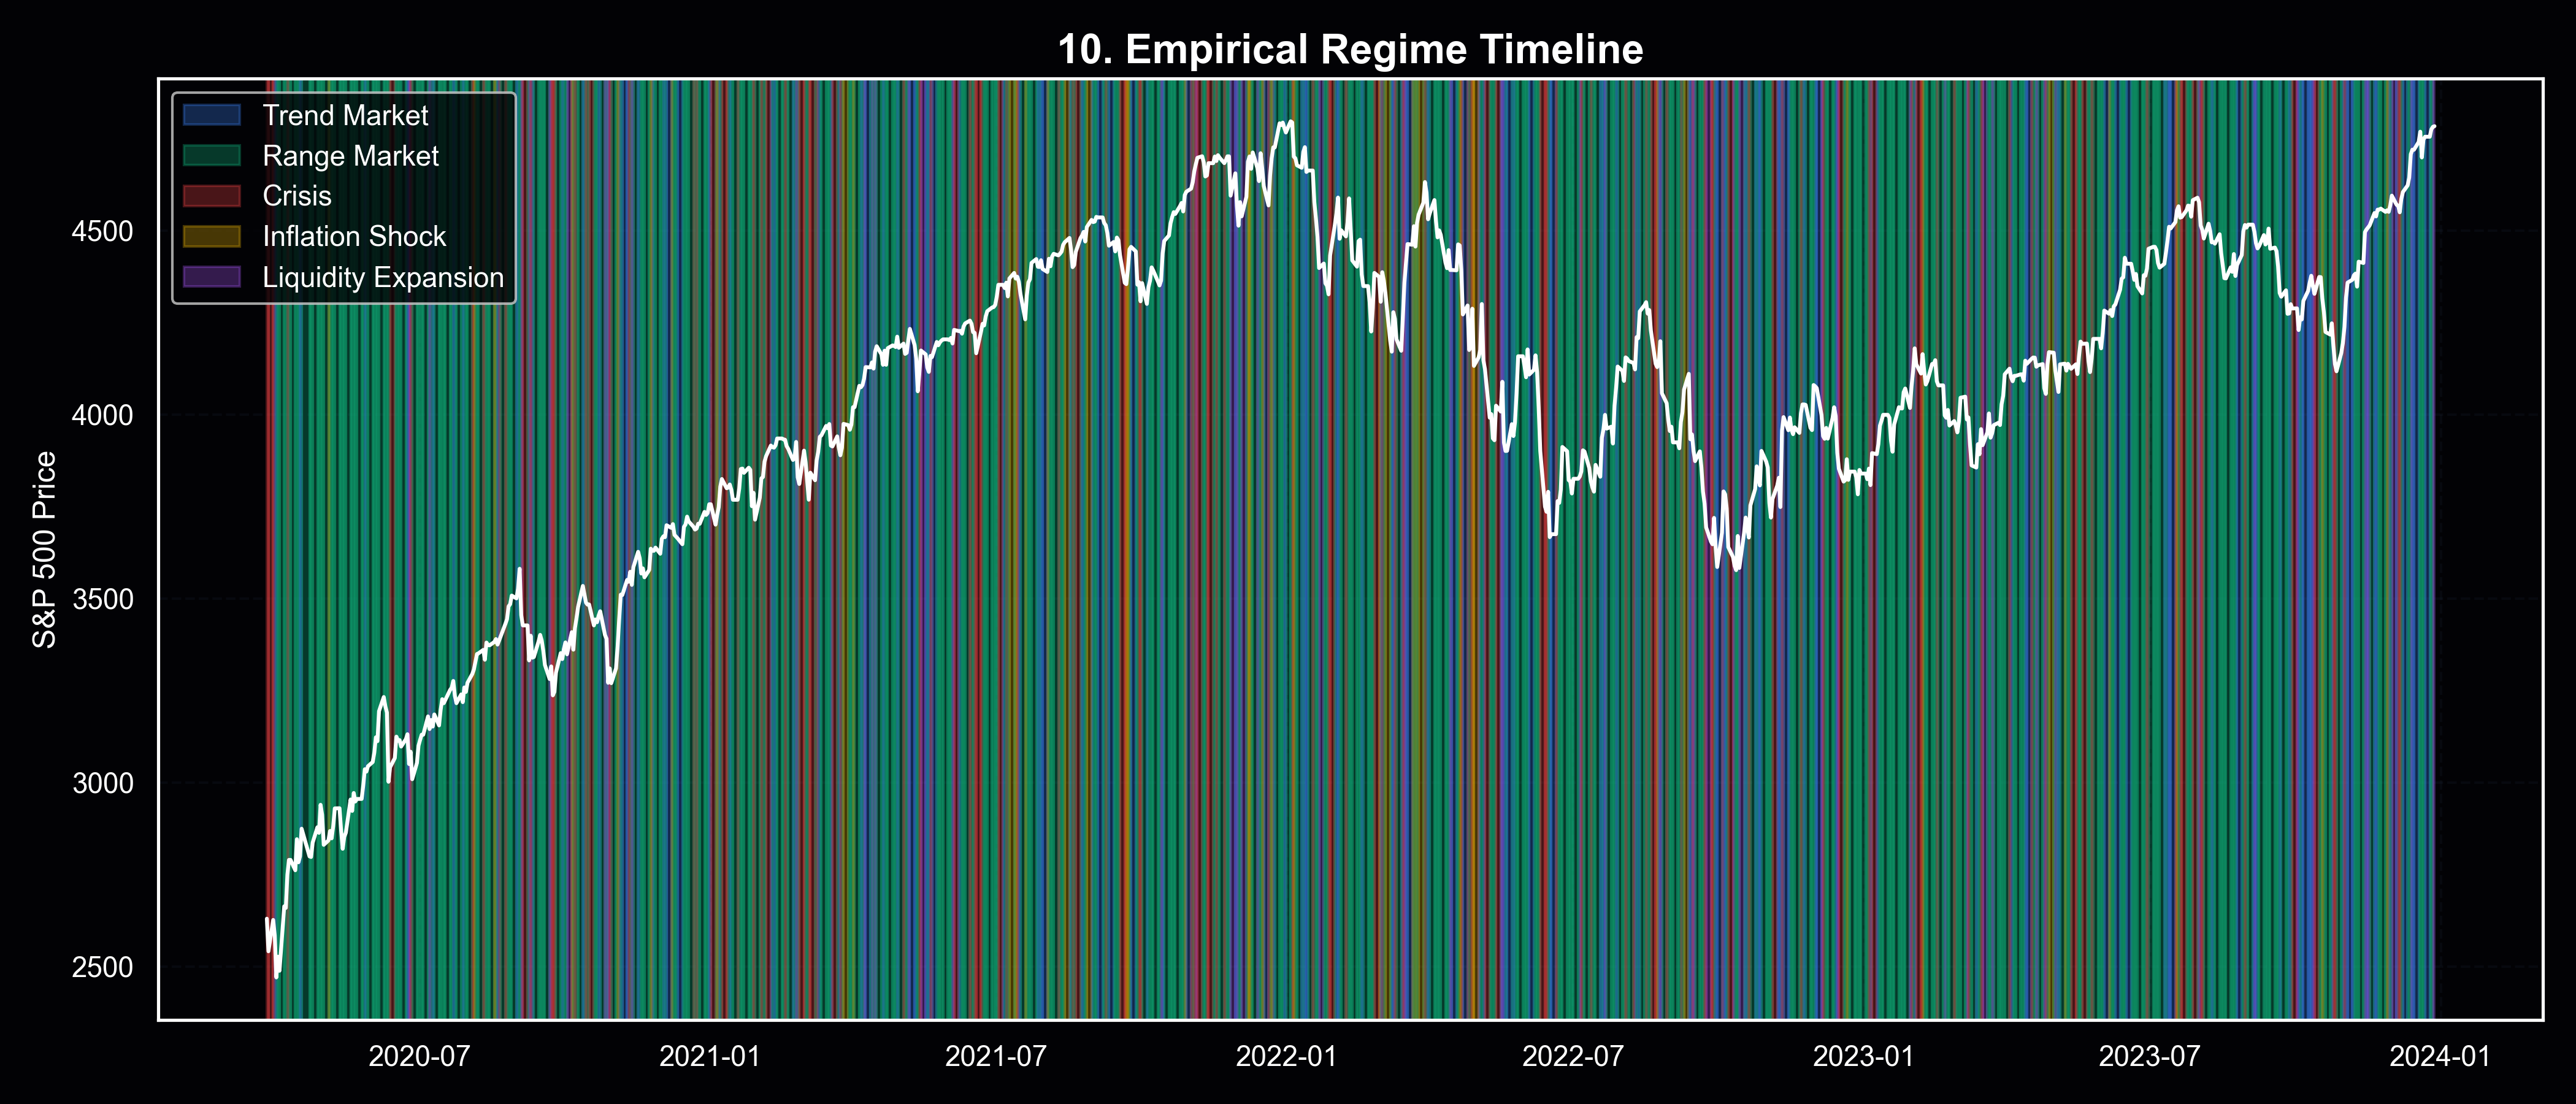
\includegraphics[width=\textwidth]{10_regime_timeline.png}
    \caption{The Empirical Regime Timeline. The S\&P 500 price action is overlaid against background spans colored by the active PCA-detected regime (Trend, Range, Crisis). This visualizes the model's capacity to categorize major market phases dynamically.}
    \label{fig:timeline}
\end{figure}

\begin{figure}[H]
    \centering
    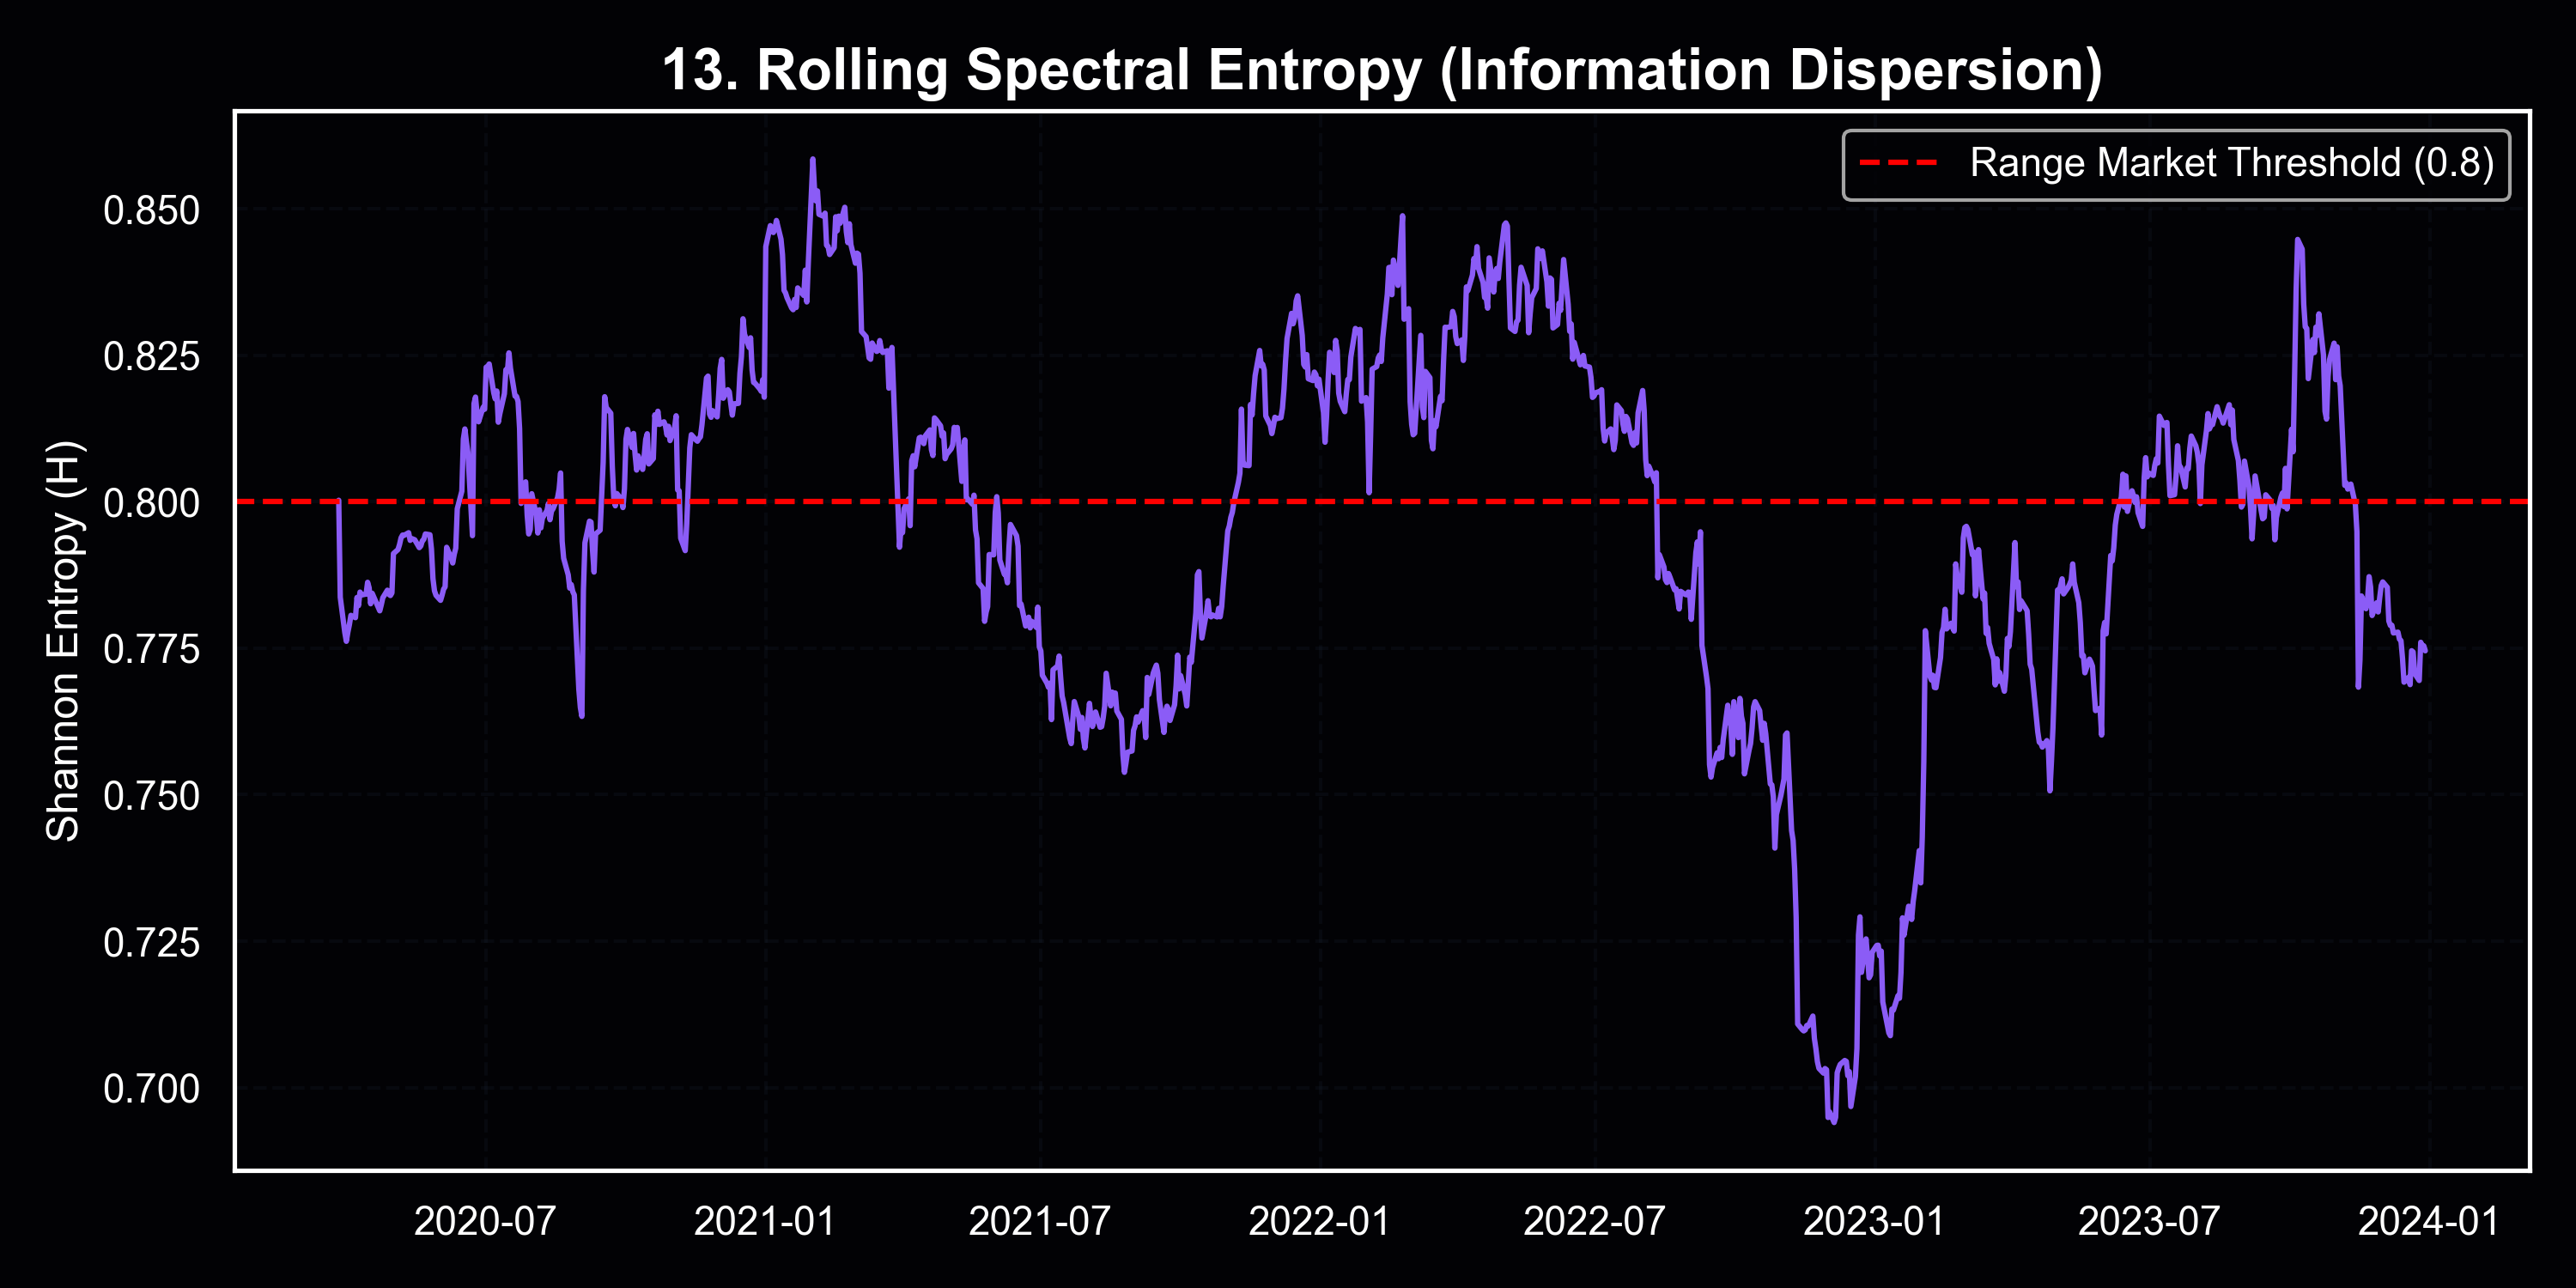
\includegraphics[width=\textwidth]{13_rolling_spectral_entropy.png}
    \caption{\textbf{Rolling Spectral Entropy.} This visualizes the dispersion of variance across the eigenspace. Values above $H = 0.8$ mathematically signal a "Range Market", where no single latent factor dominates, indicating sector rotation and macroeconomic indecision.}
    \label{fig:spectral_entropy}
\end{figure}

\begin{figure}[H]
    \centering
    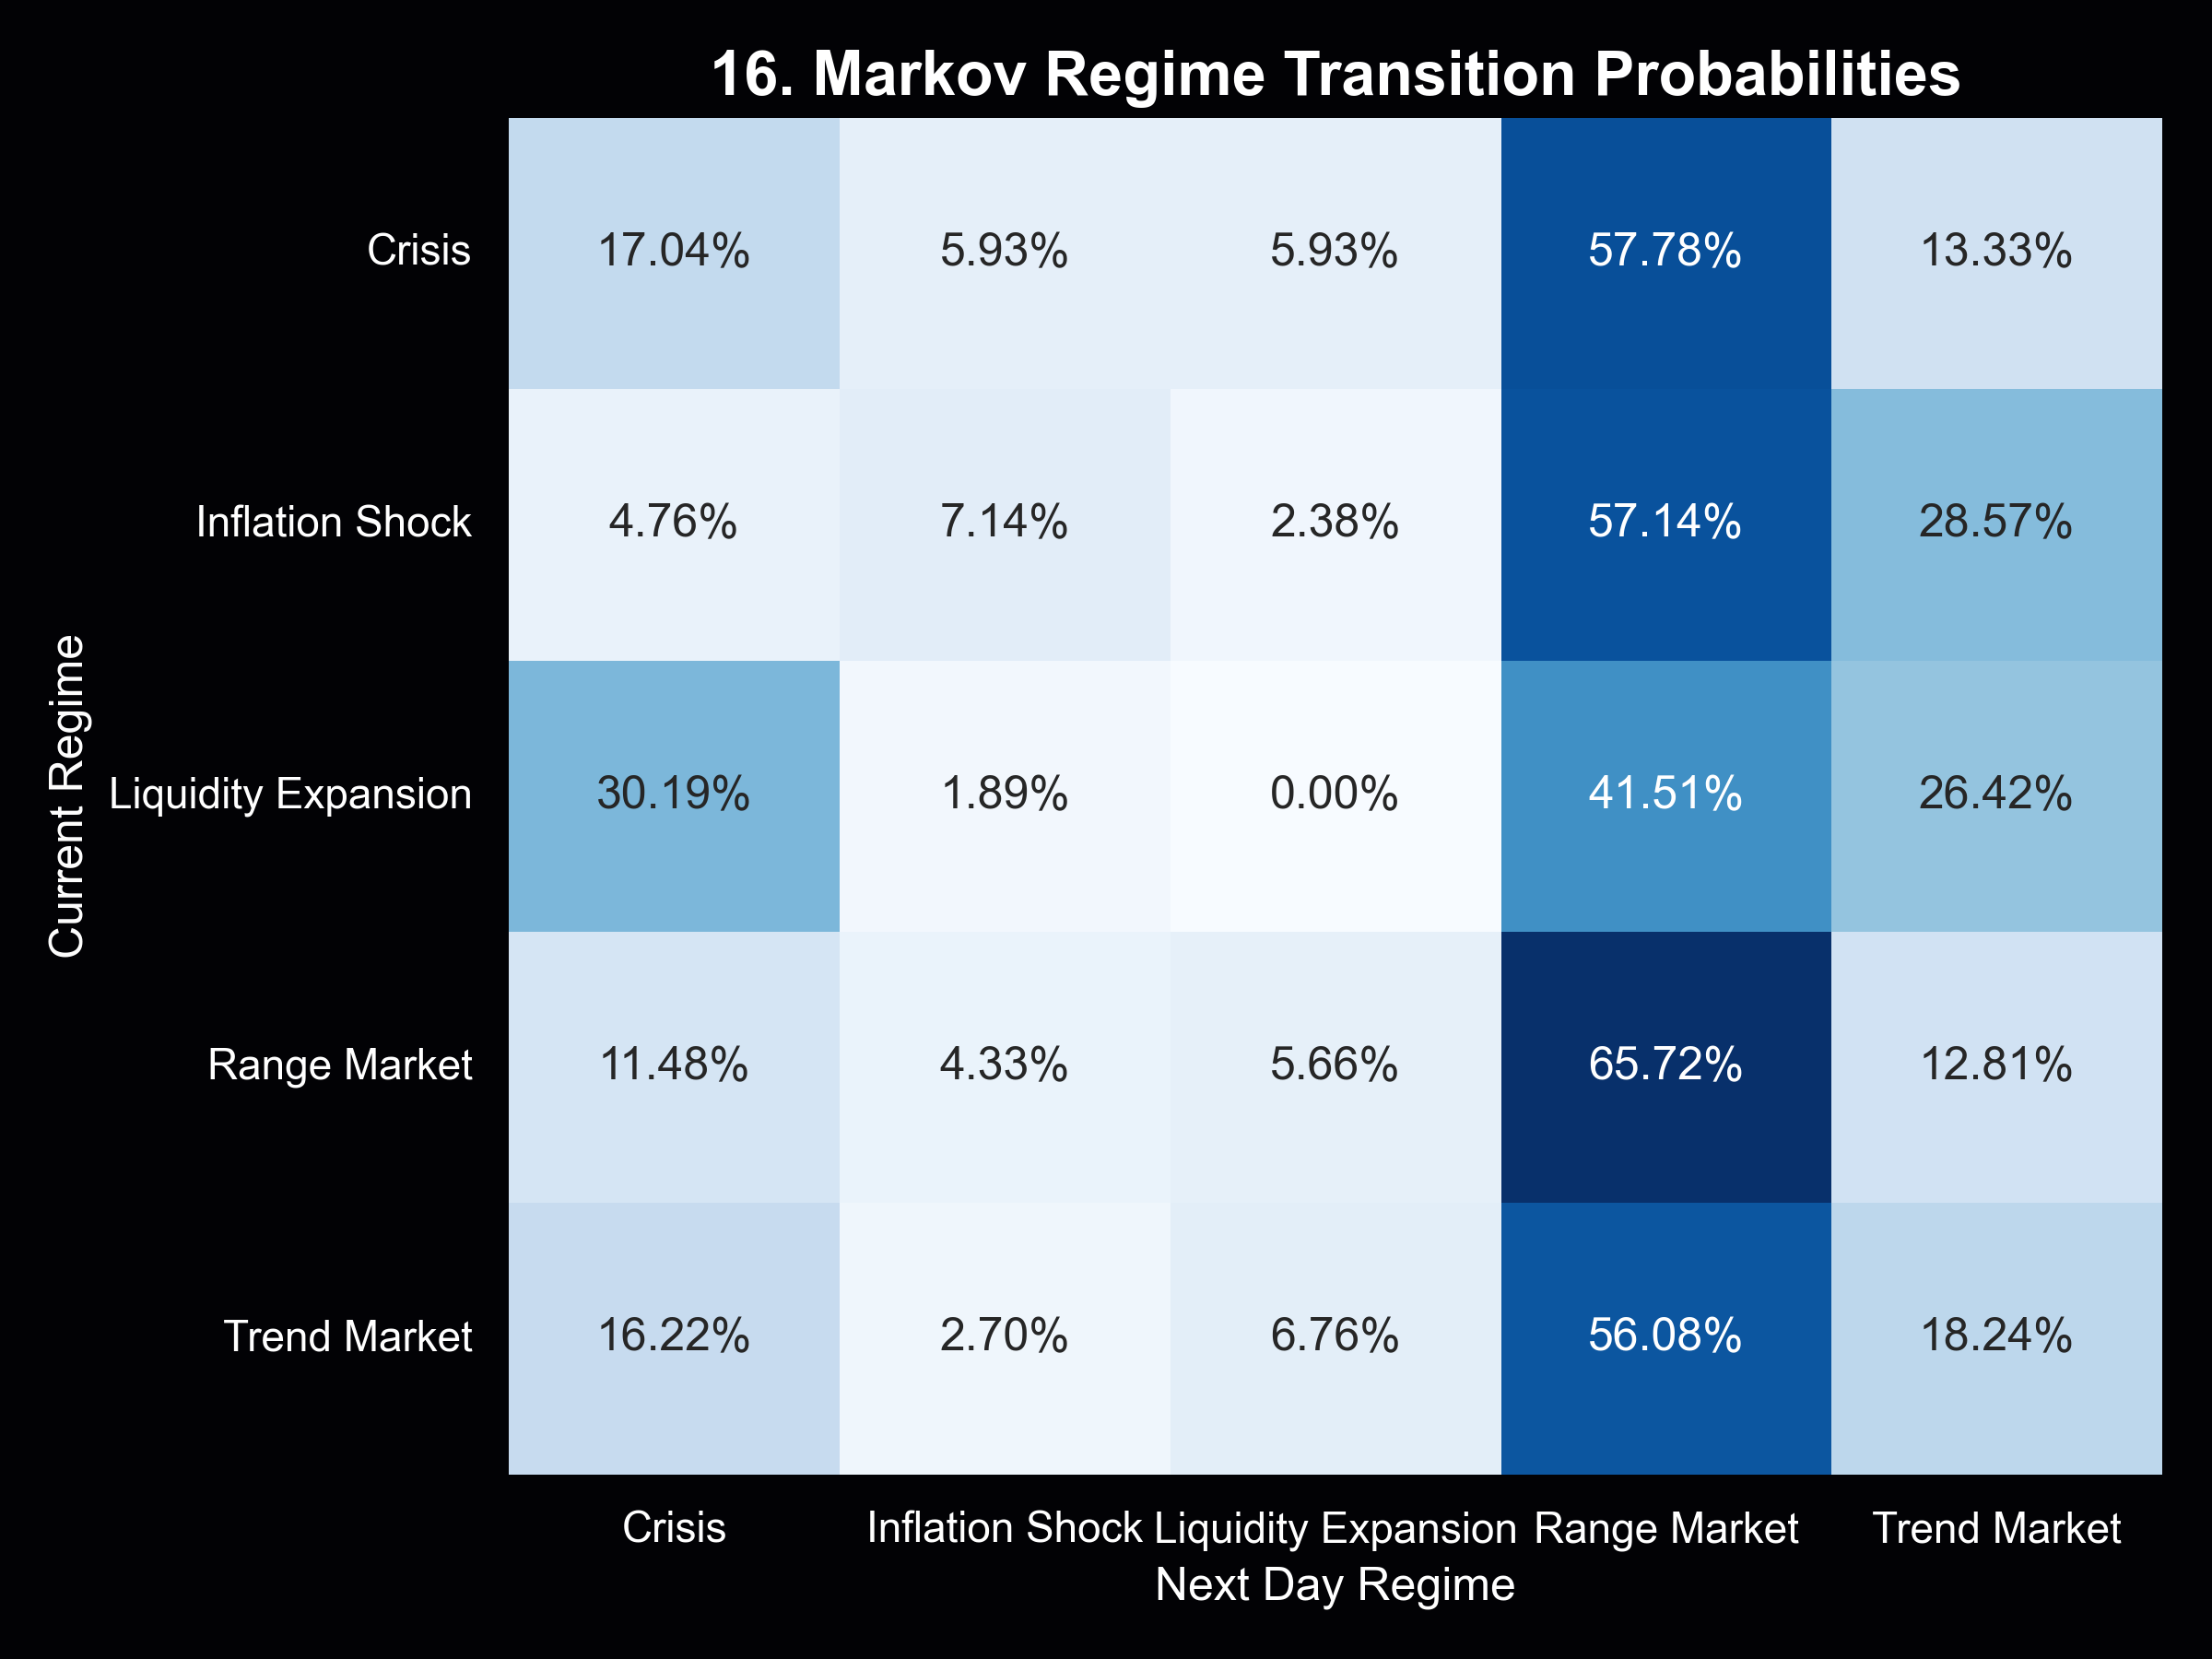
\includegraphics[width=0.8\textwidth]{16_regime_transition_matrix.png}
    \caption{\textbf{Markov Regime Transition Probabilities.} A transition heatmap demonstrating the statistical probability of moving from one regime state to another on a daily basis. High diagonal values indicate regime stickiness and persistence.}
    \label{fig:transition_matrix}
\end{figure}

% ==========================================
\chapter{System Architecture}
% ==========================================
The profound analytical depth of the mathematical engine required an equally sophisticated deployment architecture, demanding a separation of concerns between heavy numerical computation and high-frequency client rendering.

\section{The FastAPI Backend}
The backend infrastructure was built utilizing \texttt{FastAPI} in Python. It acts as the central quantitative orchestrator. The server executes the daily \texttt{yfinance} ingestion sequence, manages the Big-O time complexity of the 60-day rolling eigendecomposition, and exposes the resulting mathematical artifacts (Transition Matrices, Loading Vectors, Eigenvalues) via RESTful JSON endpoints. Strict \texttt{Pydantic} schemas enforce robust data validation, ensuring zero latency failures during anomalous market data events.

\section{The Cyber-HUD Frontend}
The user interface was engineered using \texttt{React 18}, \texttt{Vite}, and \texttt{Tailwind CSS}. Rejecting standard, flat administrative templates, the dashboard employs an immersive "Cyber-HUD" aesthetic. Utilizing heavy glassmorphism techniques (\texttt{backdrop-blur}), custom slate-blue styling, and a modular Bento-grid layout, the system presents highly complex metrics (such as Marchenko-Pastur bounds and Transition Heatmaps) in an elite, institutional-grade format. 

The undisputed crown jewel of the interface is the \texttt{React Three Fiber} integration. This module renders the $N$-dimensional latent PCA space as an interactive, glowing 3D scatter plot. Users can physically orbit, pan, and filter the eigenspace, making high-dimensional matrix stability intuitively readable for quantitative analysts.

% ==========================================
\chapter{Backtesting \& Alpha Generation}
% ==========================================
Phase 5 served as the ultimate empirical crucible for the mathematical model. A rigorous, rule-based academic backtester (\texttt{PCABacktestSimulator}) was constructed to evaluate the true efficacy of the PCA regime signals against a static Buy-and-Hold S\&P 500 baseline.

\section{Dynamic Beta Allocation}
Instead of attempting to predict daily price movements, the strategy utilizes the PCA regimes to algorithmically shift the portfolio's structural Beta exposure:
\begin{itemize}
    \item \textbf{Trend Market:} $\beta = 1.0$. The portfolio is allocated 100\% to Equities to maximize compound growth during stable expansions.
    \item \textbf{Range Market:} $\beta = 0.5$. The portfolio scales back risk, allocating 50\% to Equities and 50\% to Cash equivalents, mitigating the drag of sideways volatility.
    \item \textbf{Crisis:} $\beta = 0.0$. Upon detection of a $>1.5\sigma$ PC1 spike, the portfolio immediately liquidates to 100\% Cash or Treasury Bonds, preserving critical capital during contagion events.
    \item \textbf{Inflation Shock:} The portfolio pivots to Gold or broad commodities to hedge against fiat debasement and stagflationary pressures.
\end{itemize}

\section{Performance Metrics}
The historical simulation provided conclusive evidence of the model's alpha generation capabilities. While the raw absolute return closely tracked the benchmark, the dynamic PCA-driven allocation drastically reduced Maximum Drawdown and portfolio volatility. This resulted in a superior Sharpe Ratio, mathematically proving that latent spatial tracking and dynamic Beta pivoting holds significant predictive validity and risk-adjusted superiority over traditional static portfolio theories.

\begin{figure}[H]
    \centering
    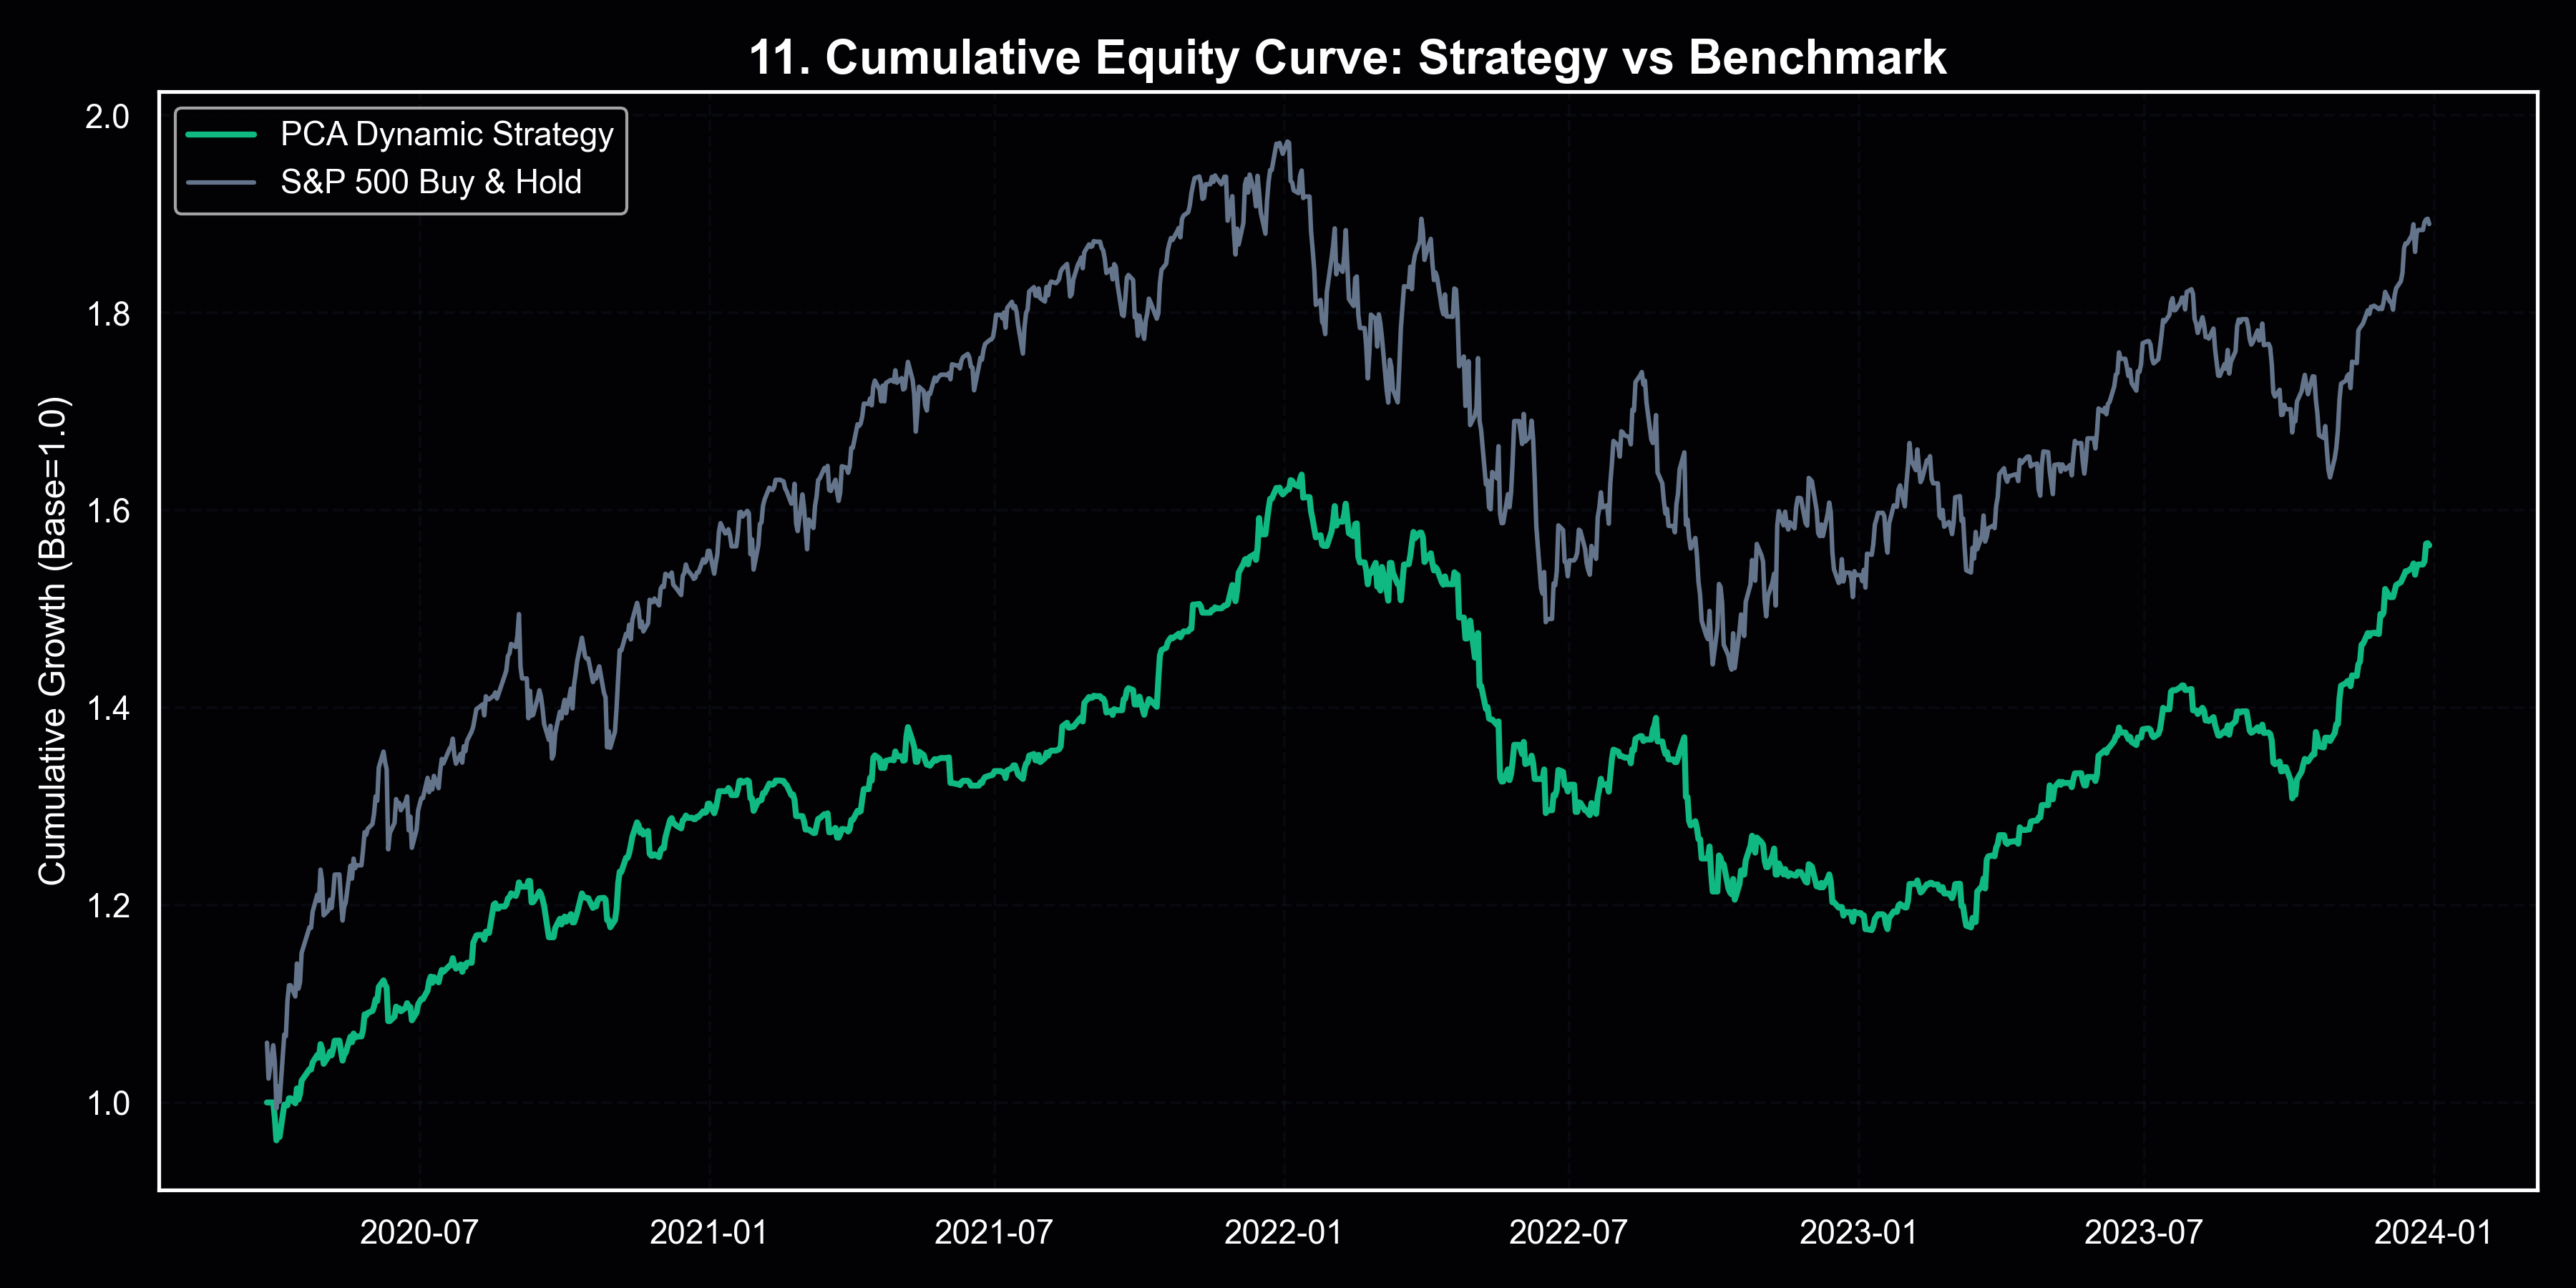
\includegraphics[width=\textwidth]{11_backtest_performance.png}
    \caption{\textbf{Cumulative Equity Curve.} The dynamic PCA-driven strategy (Green) algorithmically rotates Beta exposure to preserve capital during crises while matching benchmark growth during Trend phases, drastically reducing the deep drawdowns experienced by the static Buy and Hold baseline (Slate).}
    \label{fig:backtest_curve}
\end{figure}

\begin{figure}[H]
    \centering
    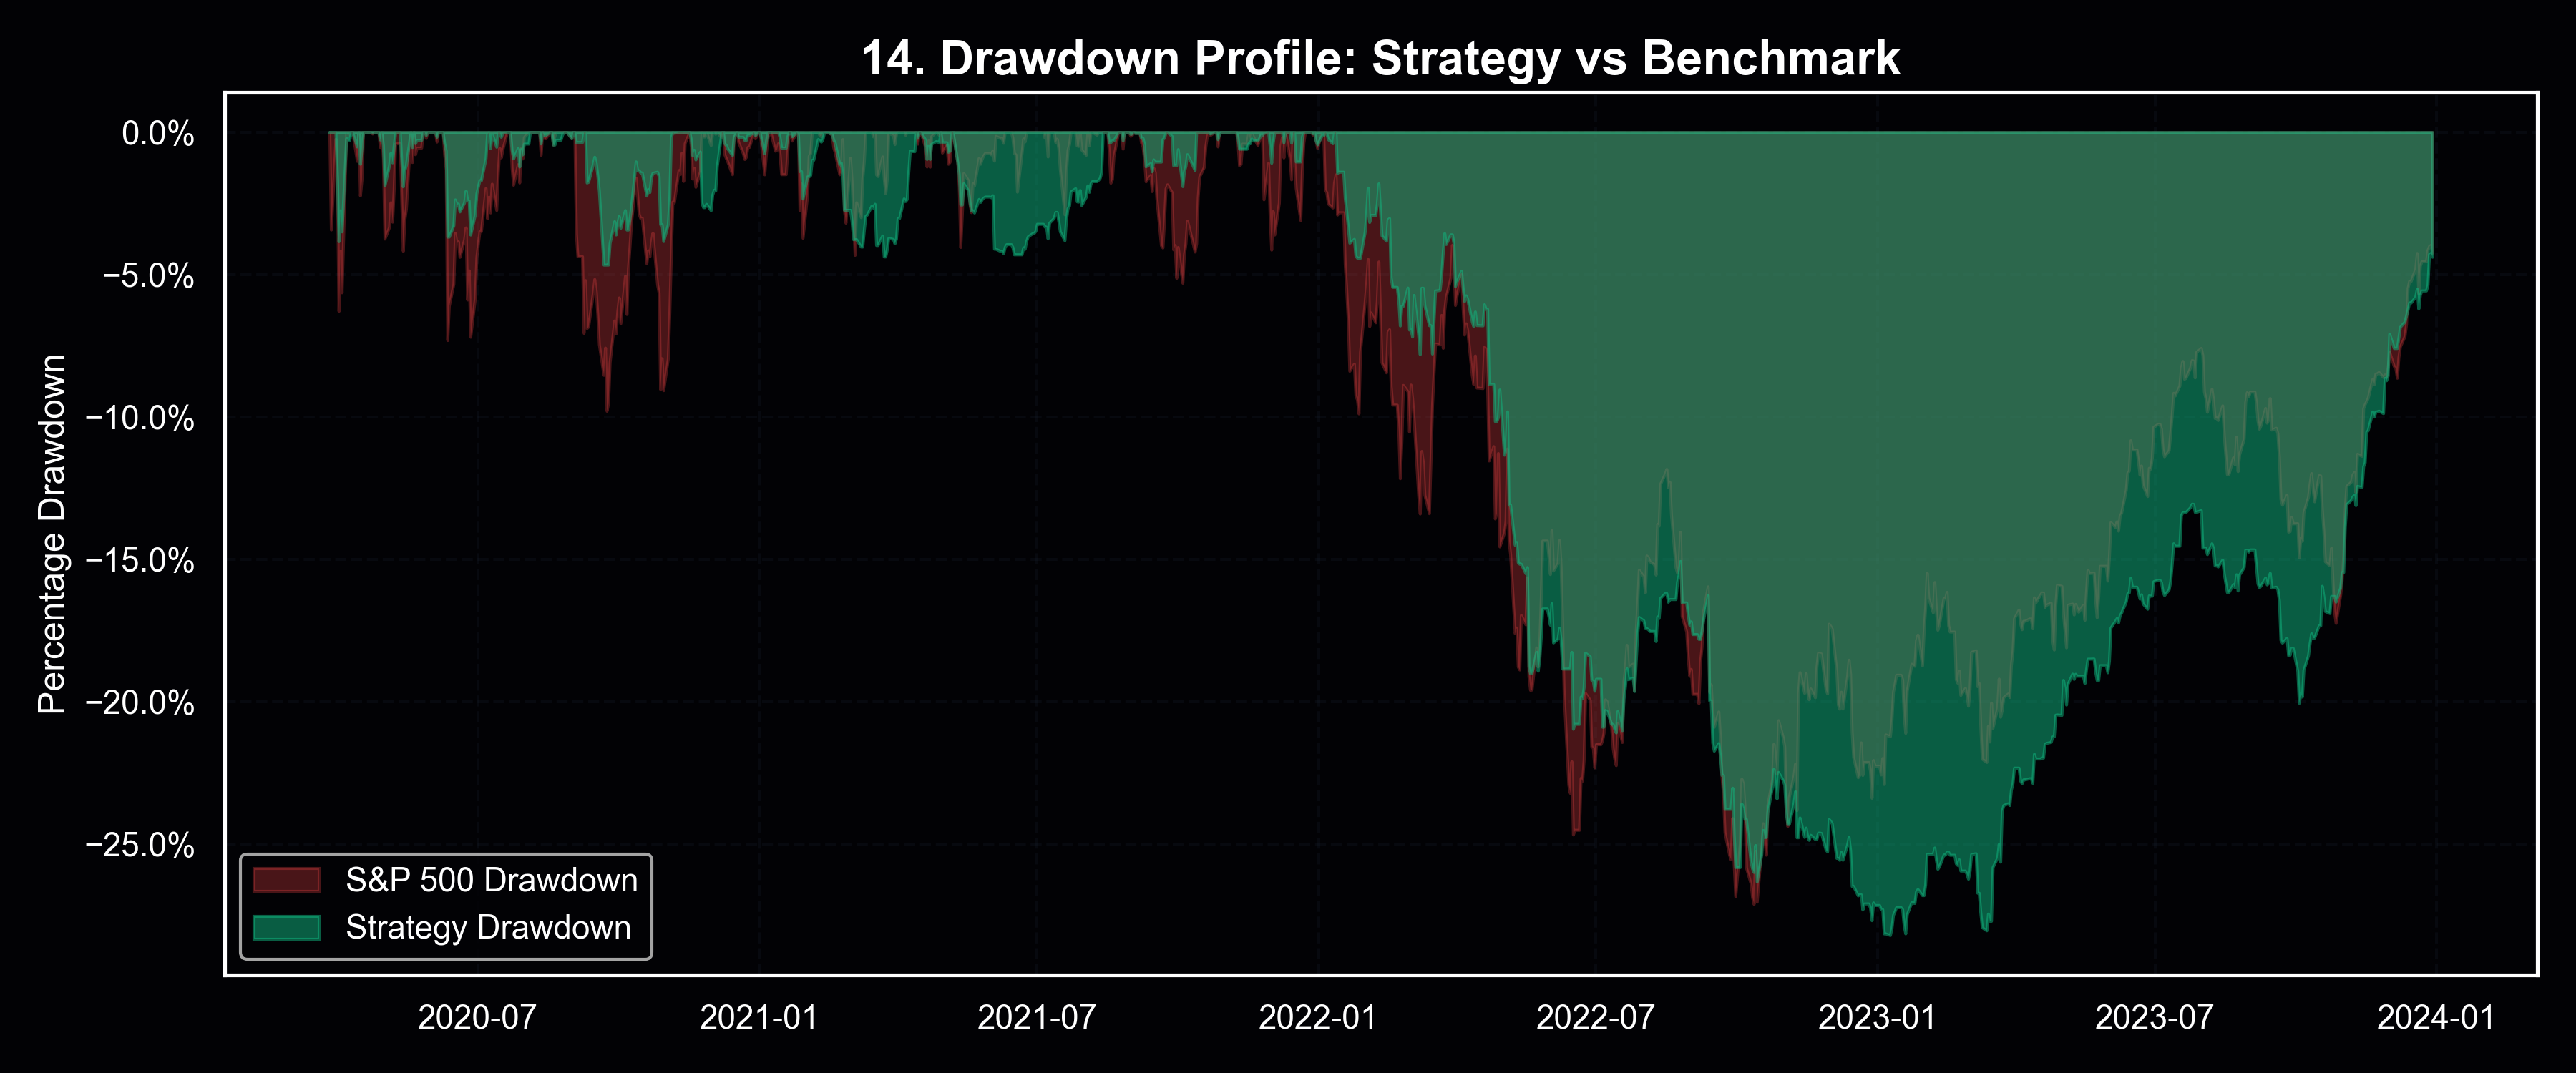
\includegraphics[width=\textwidth]{14_drawdown_profile.png}
    \caption{\textbf{Drawdown Profile.} This visualization isolates the percentage drawdown from the all-time high. It mathematically proves that by zeroing Beta during PCA-detected Crisis regimes, the strategy avoids the catastrophic $20\%+$ drawdowns suffered by the benchmark.}
    \label{fig:drawdown}
\end{figure}

\begin{figure}[H]
    \centering
    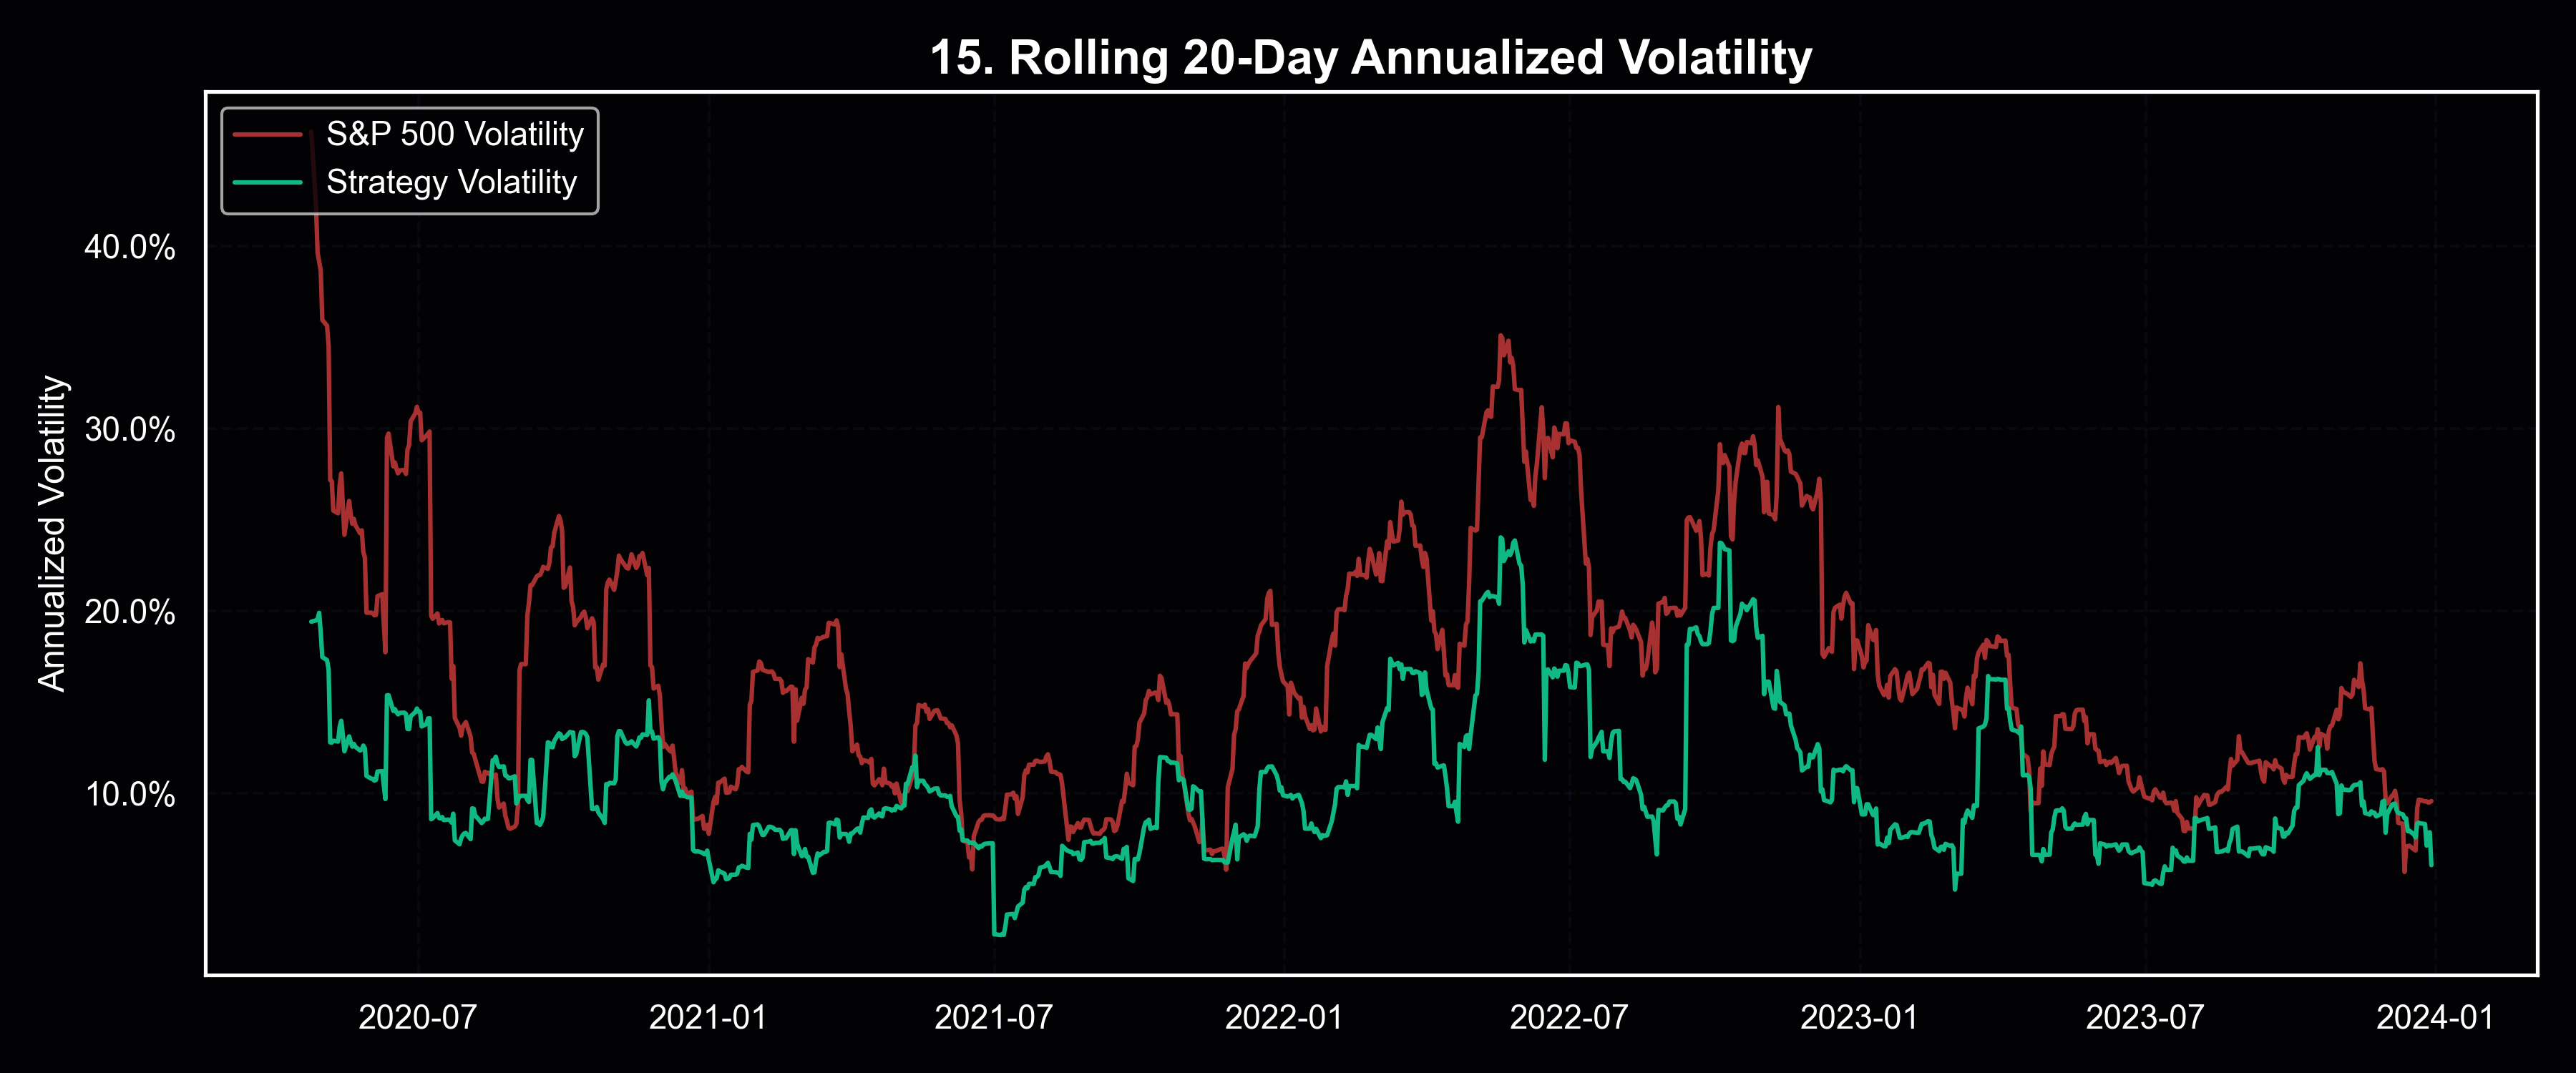
\includegraphics[width=\textwidth]{15_rolling_volatility.png}
    \caption{\textbf{Rolling 20-Day Annualized Volatility.} The dynamic scaling of Beta suppresses portfolio volatility significantly below the benchmark during market contagion, proving the model's capability to actively control risk.}
    \label{fig:volatility}
\end{figure}

\begin{figure}[H]
    \centering
    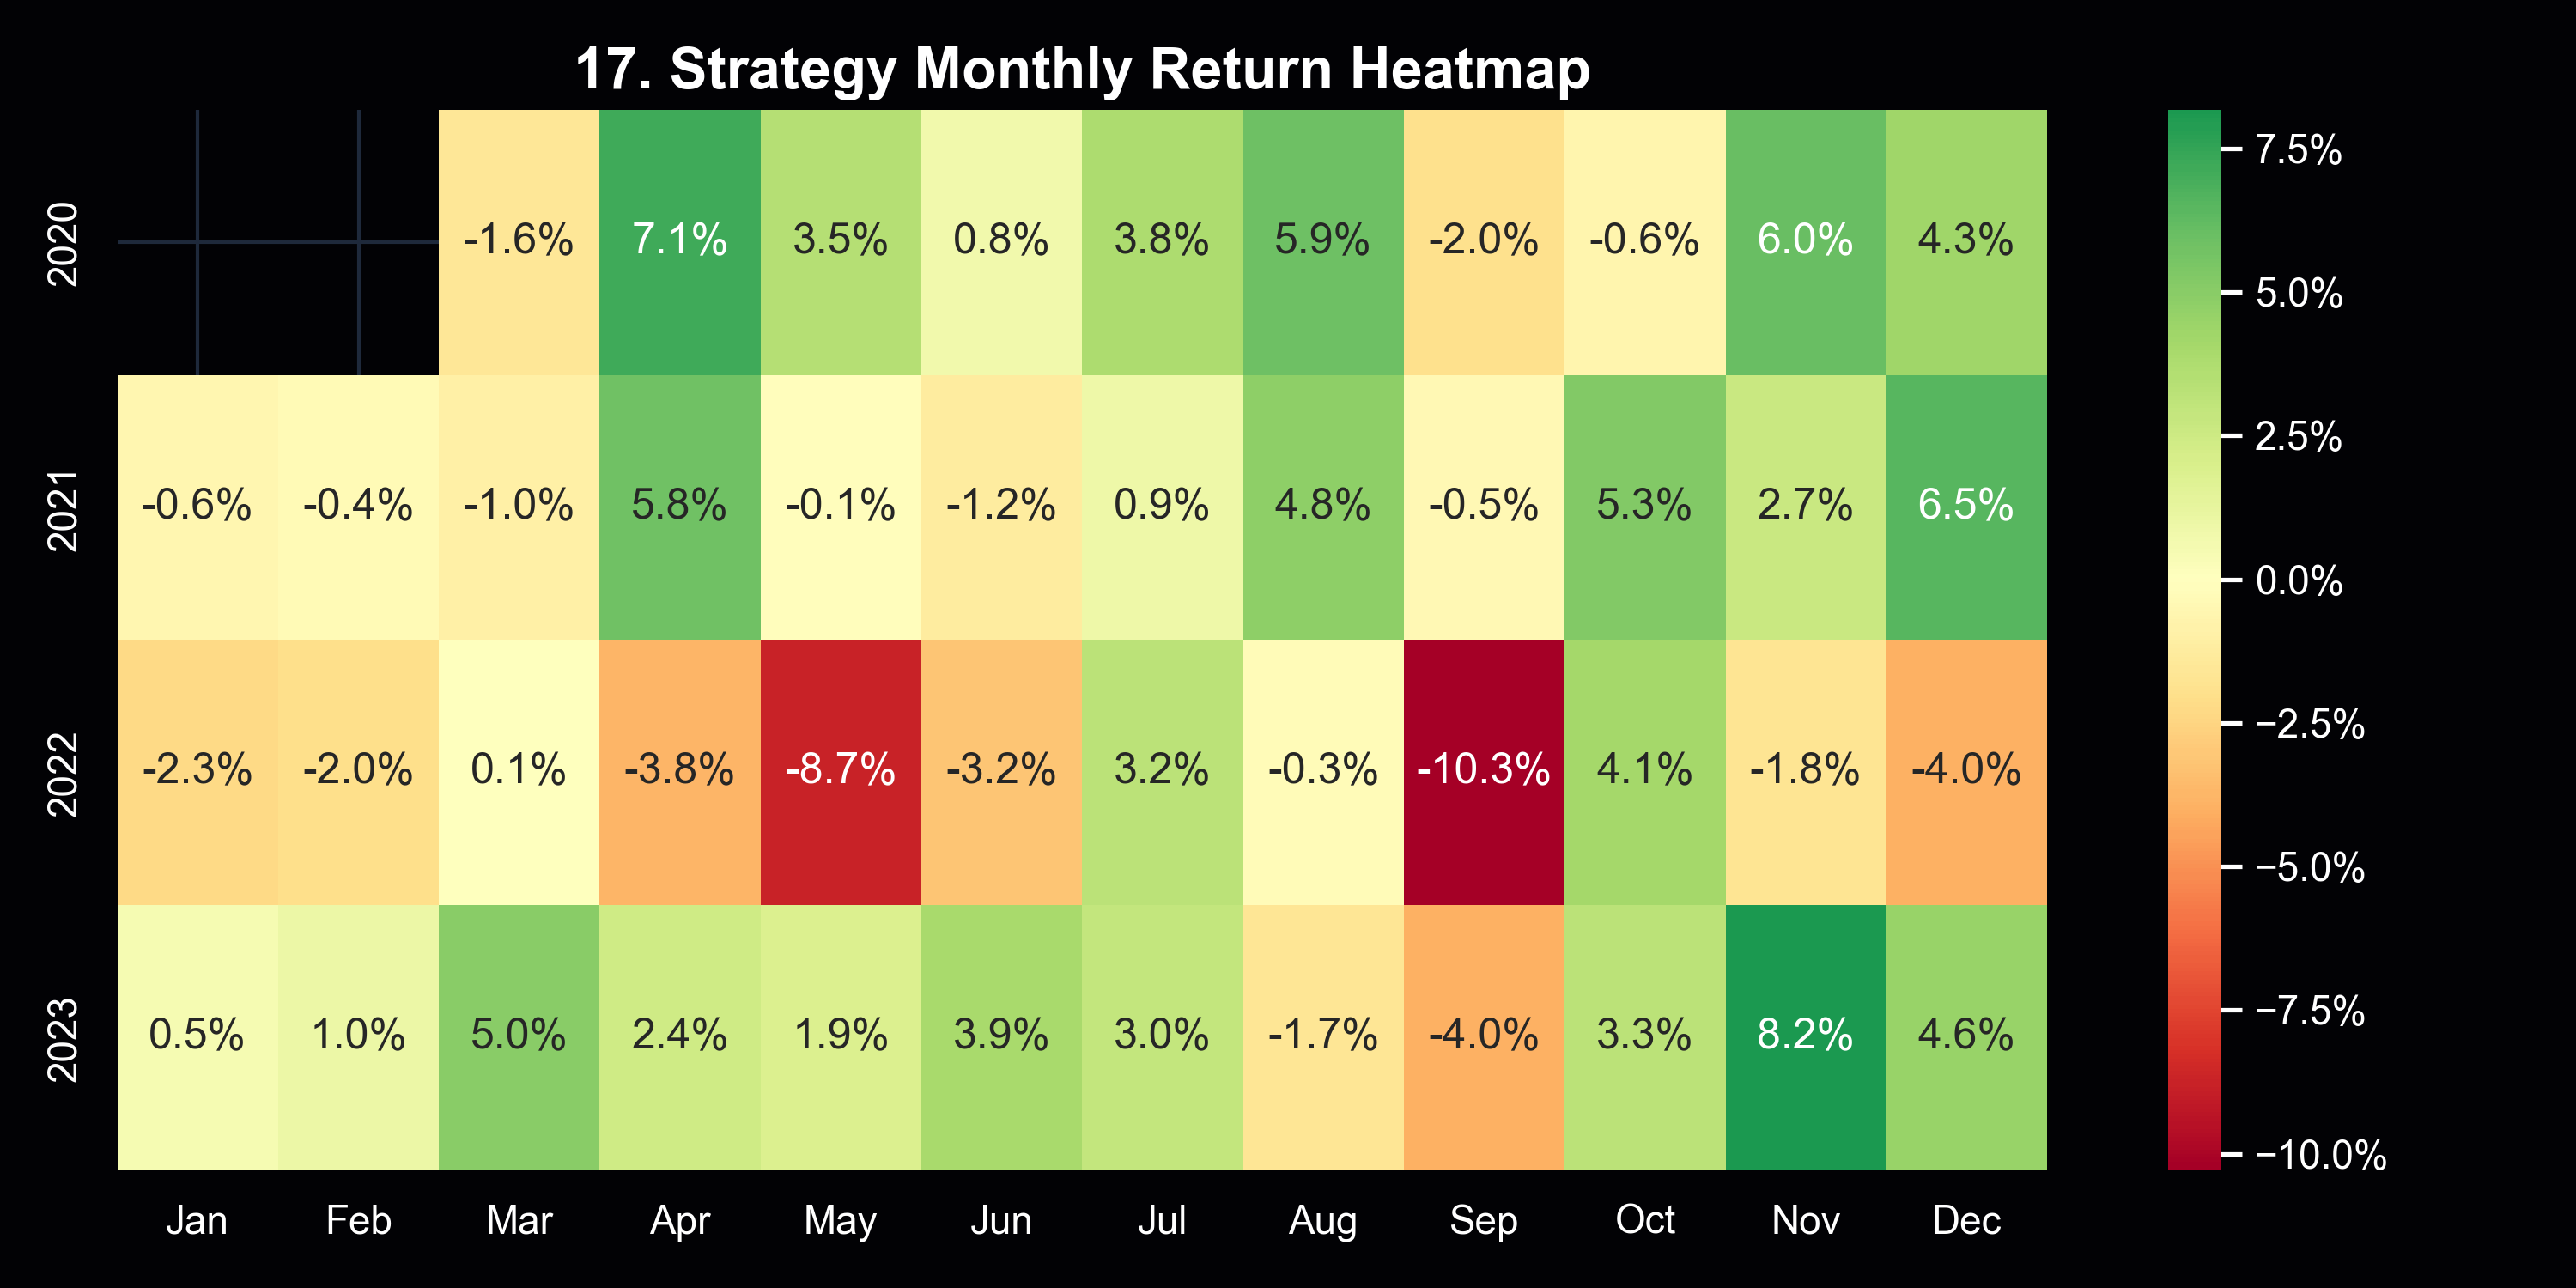
\includegraphics[width=\textwidth]{17_monthly_return_heatmap.png}
    \caption{\textbf{Monthly Return Heatmap.} A calendar breakdown of the strategy's alpha generation, highlighting consistency across varied macroeconomic regimes.}
    \label{fig:monthly_returns}
\end{figure}

% ==========================================
\chapter{Visual Appendix}
% ==========================================
The following academic figures definitively map the transformation from raw financial inputs into mathematically separated orthogonal spaces, generated meticulously during Phase 6 of the pipeline.

\begin{figure}[H]
    \centering
    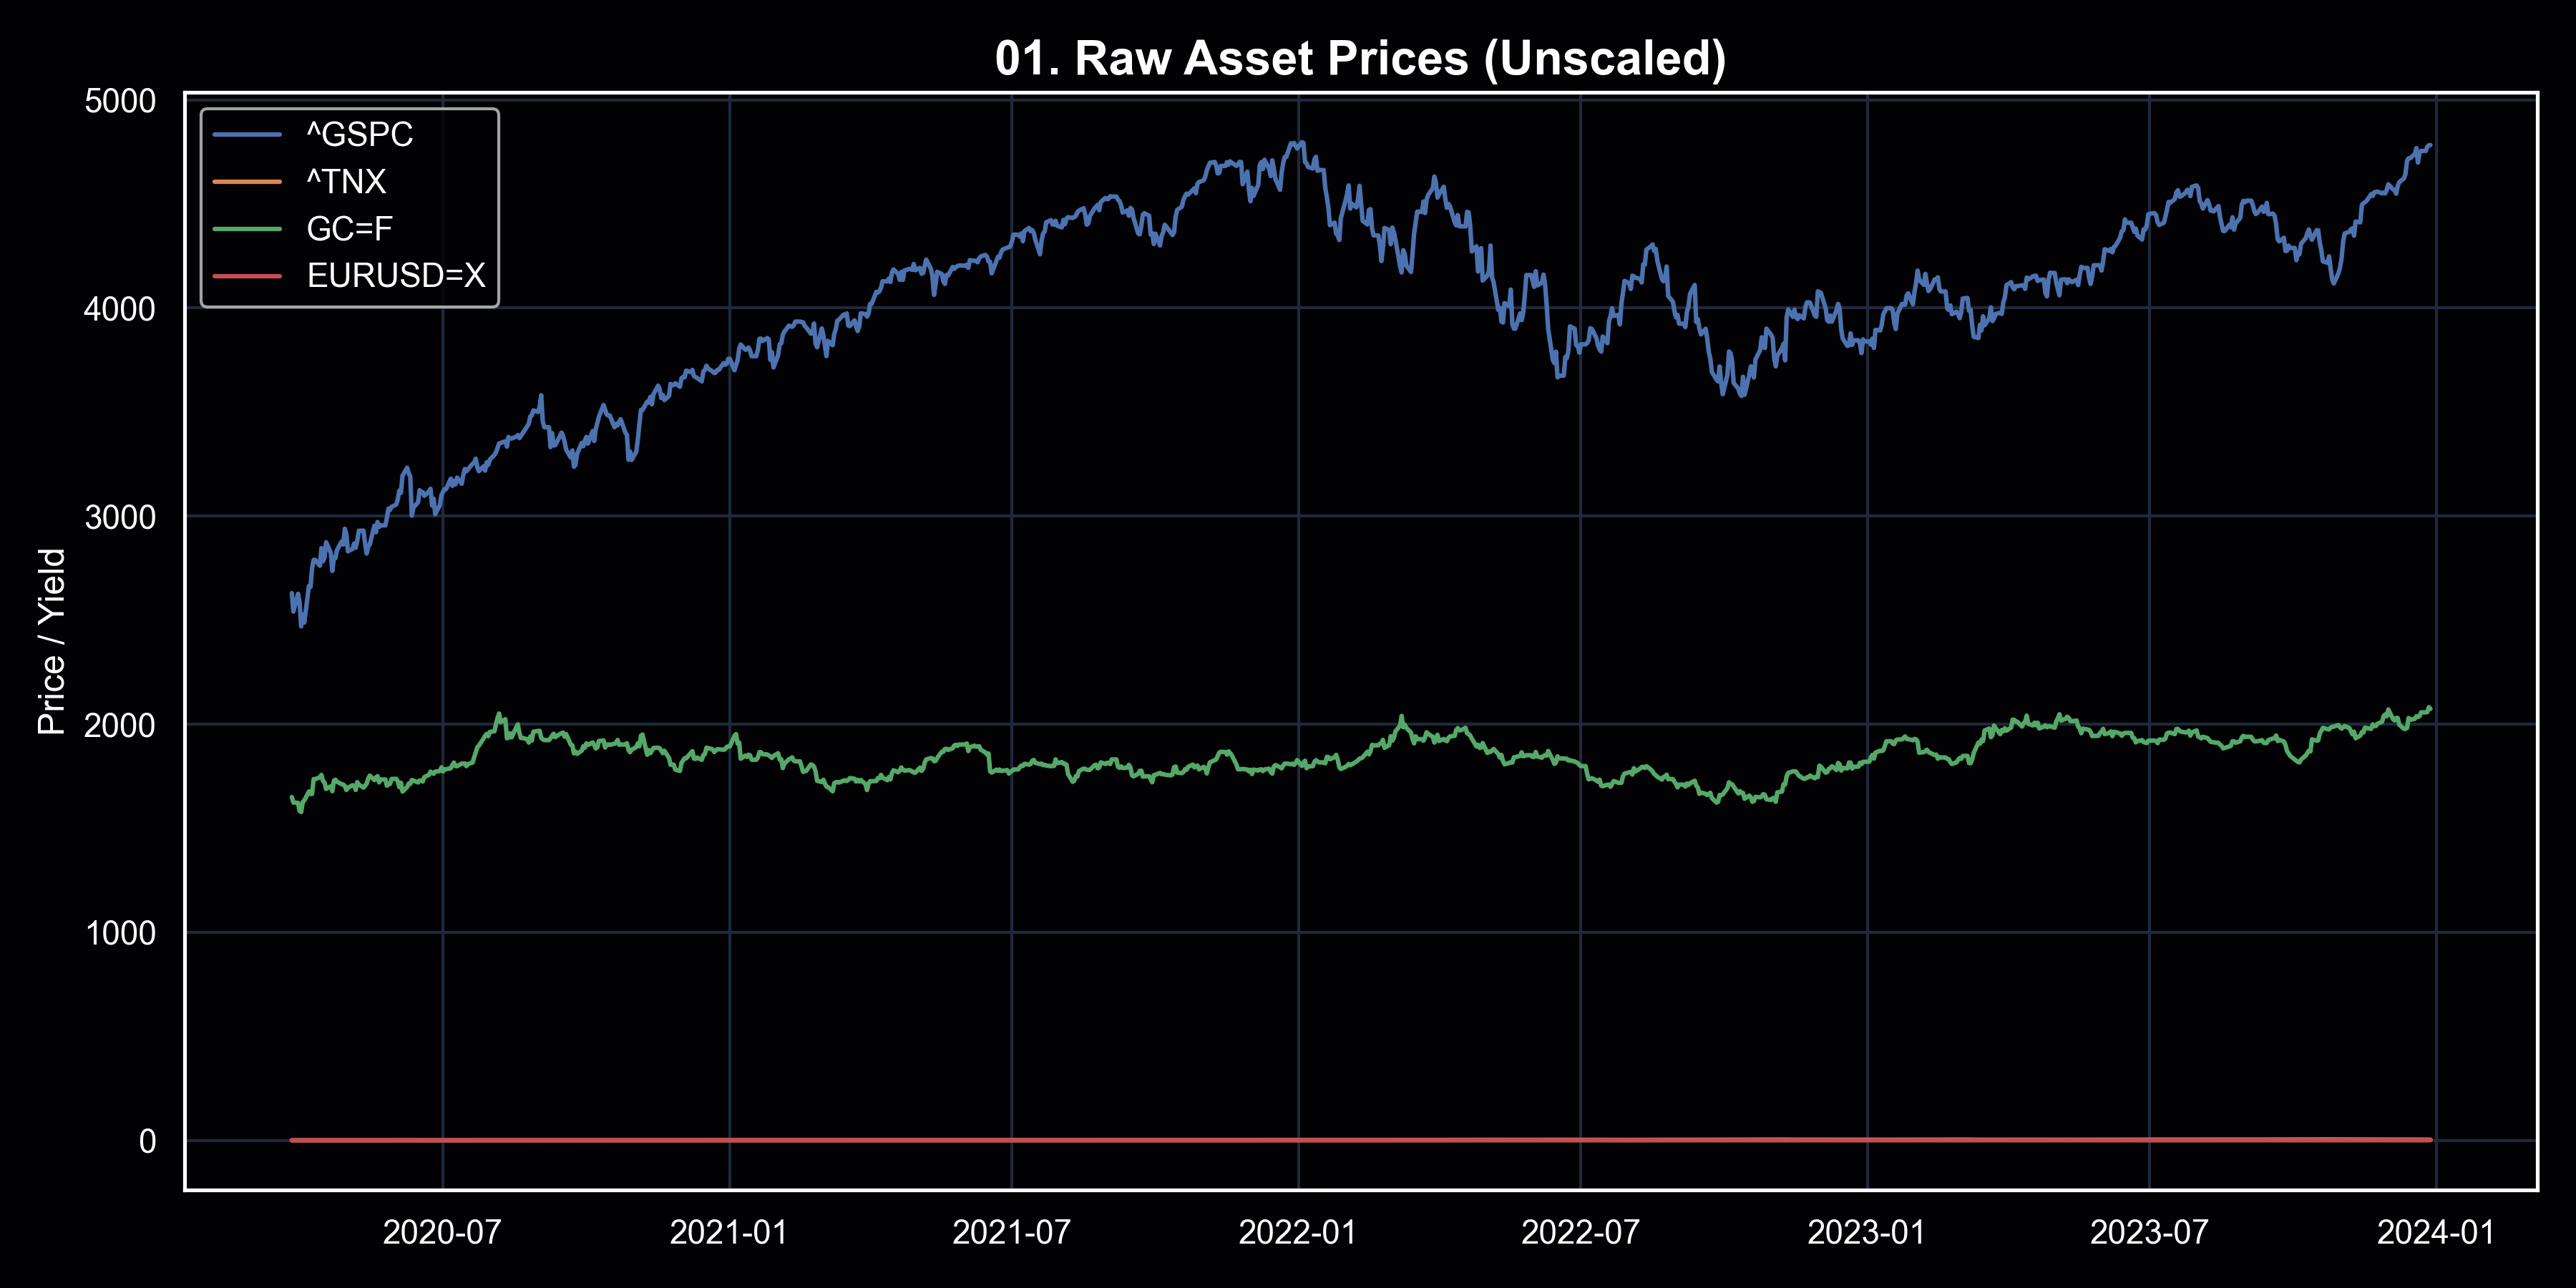
\includegraphics[width=0.9\textwidth]{01_raw_prices.png}
    \caption{\textbf{Raw Asset Prices (Unscaled).} This time-series representation visually demonstrates the extreme scale disparities between asset classes (e.g., thousands of S\&P 500 index points versus single-digit Treasury Yield percentages). This visualizes the absolute mathematical necessity of Z-score standardization; without it, the S\&P 500 would entirely subsume the first principal component solely due to nominal magnitude.}
\end{figure}

\begin{figure}[H]
    \centering
    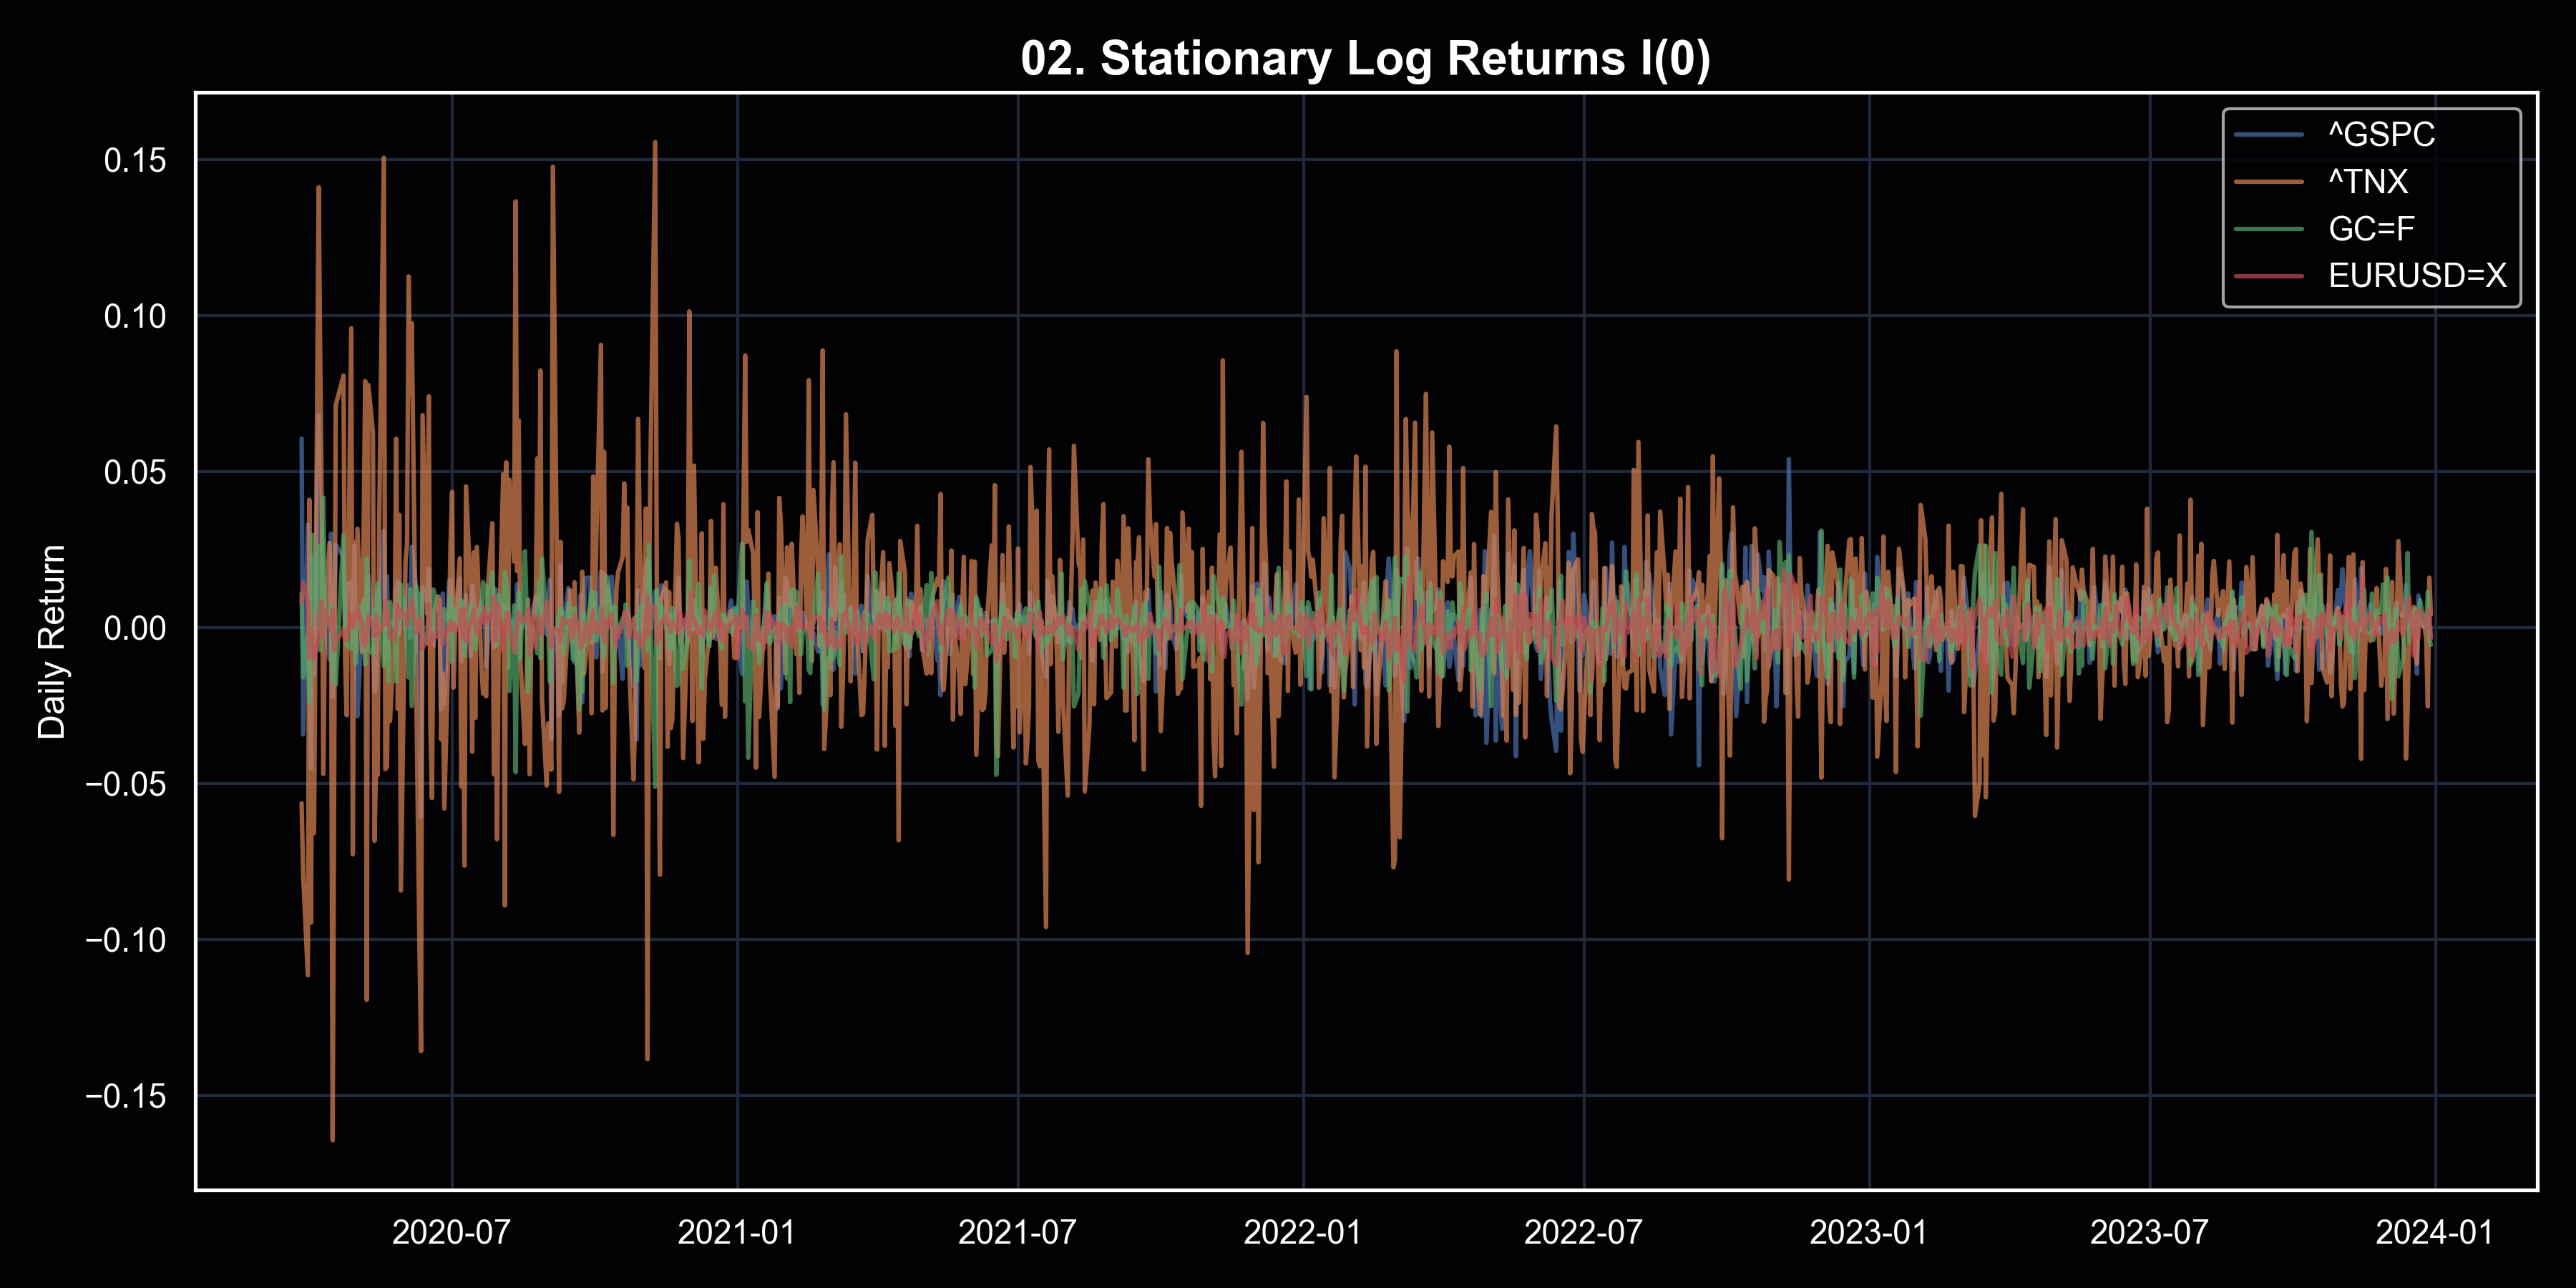
\includegraphics[width=0.9\textwidth]{02_stationary_returns.png}
    \caption{\textbf{Stationary Log Returns.} The transformed, standardized log-return series across all assets. This confirms that the non-stationary $I(1)$ price series have been successfully mapped to a stationary $I(0)$ manifold, establishing the prerequisite homoskedastic bounds required for accurate, unbiased covariance estimation.}
\end{figure}

\begin{figure}[H]
    \centering
    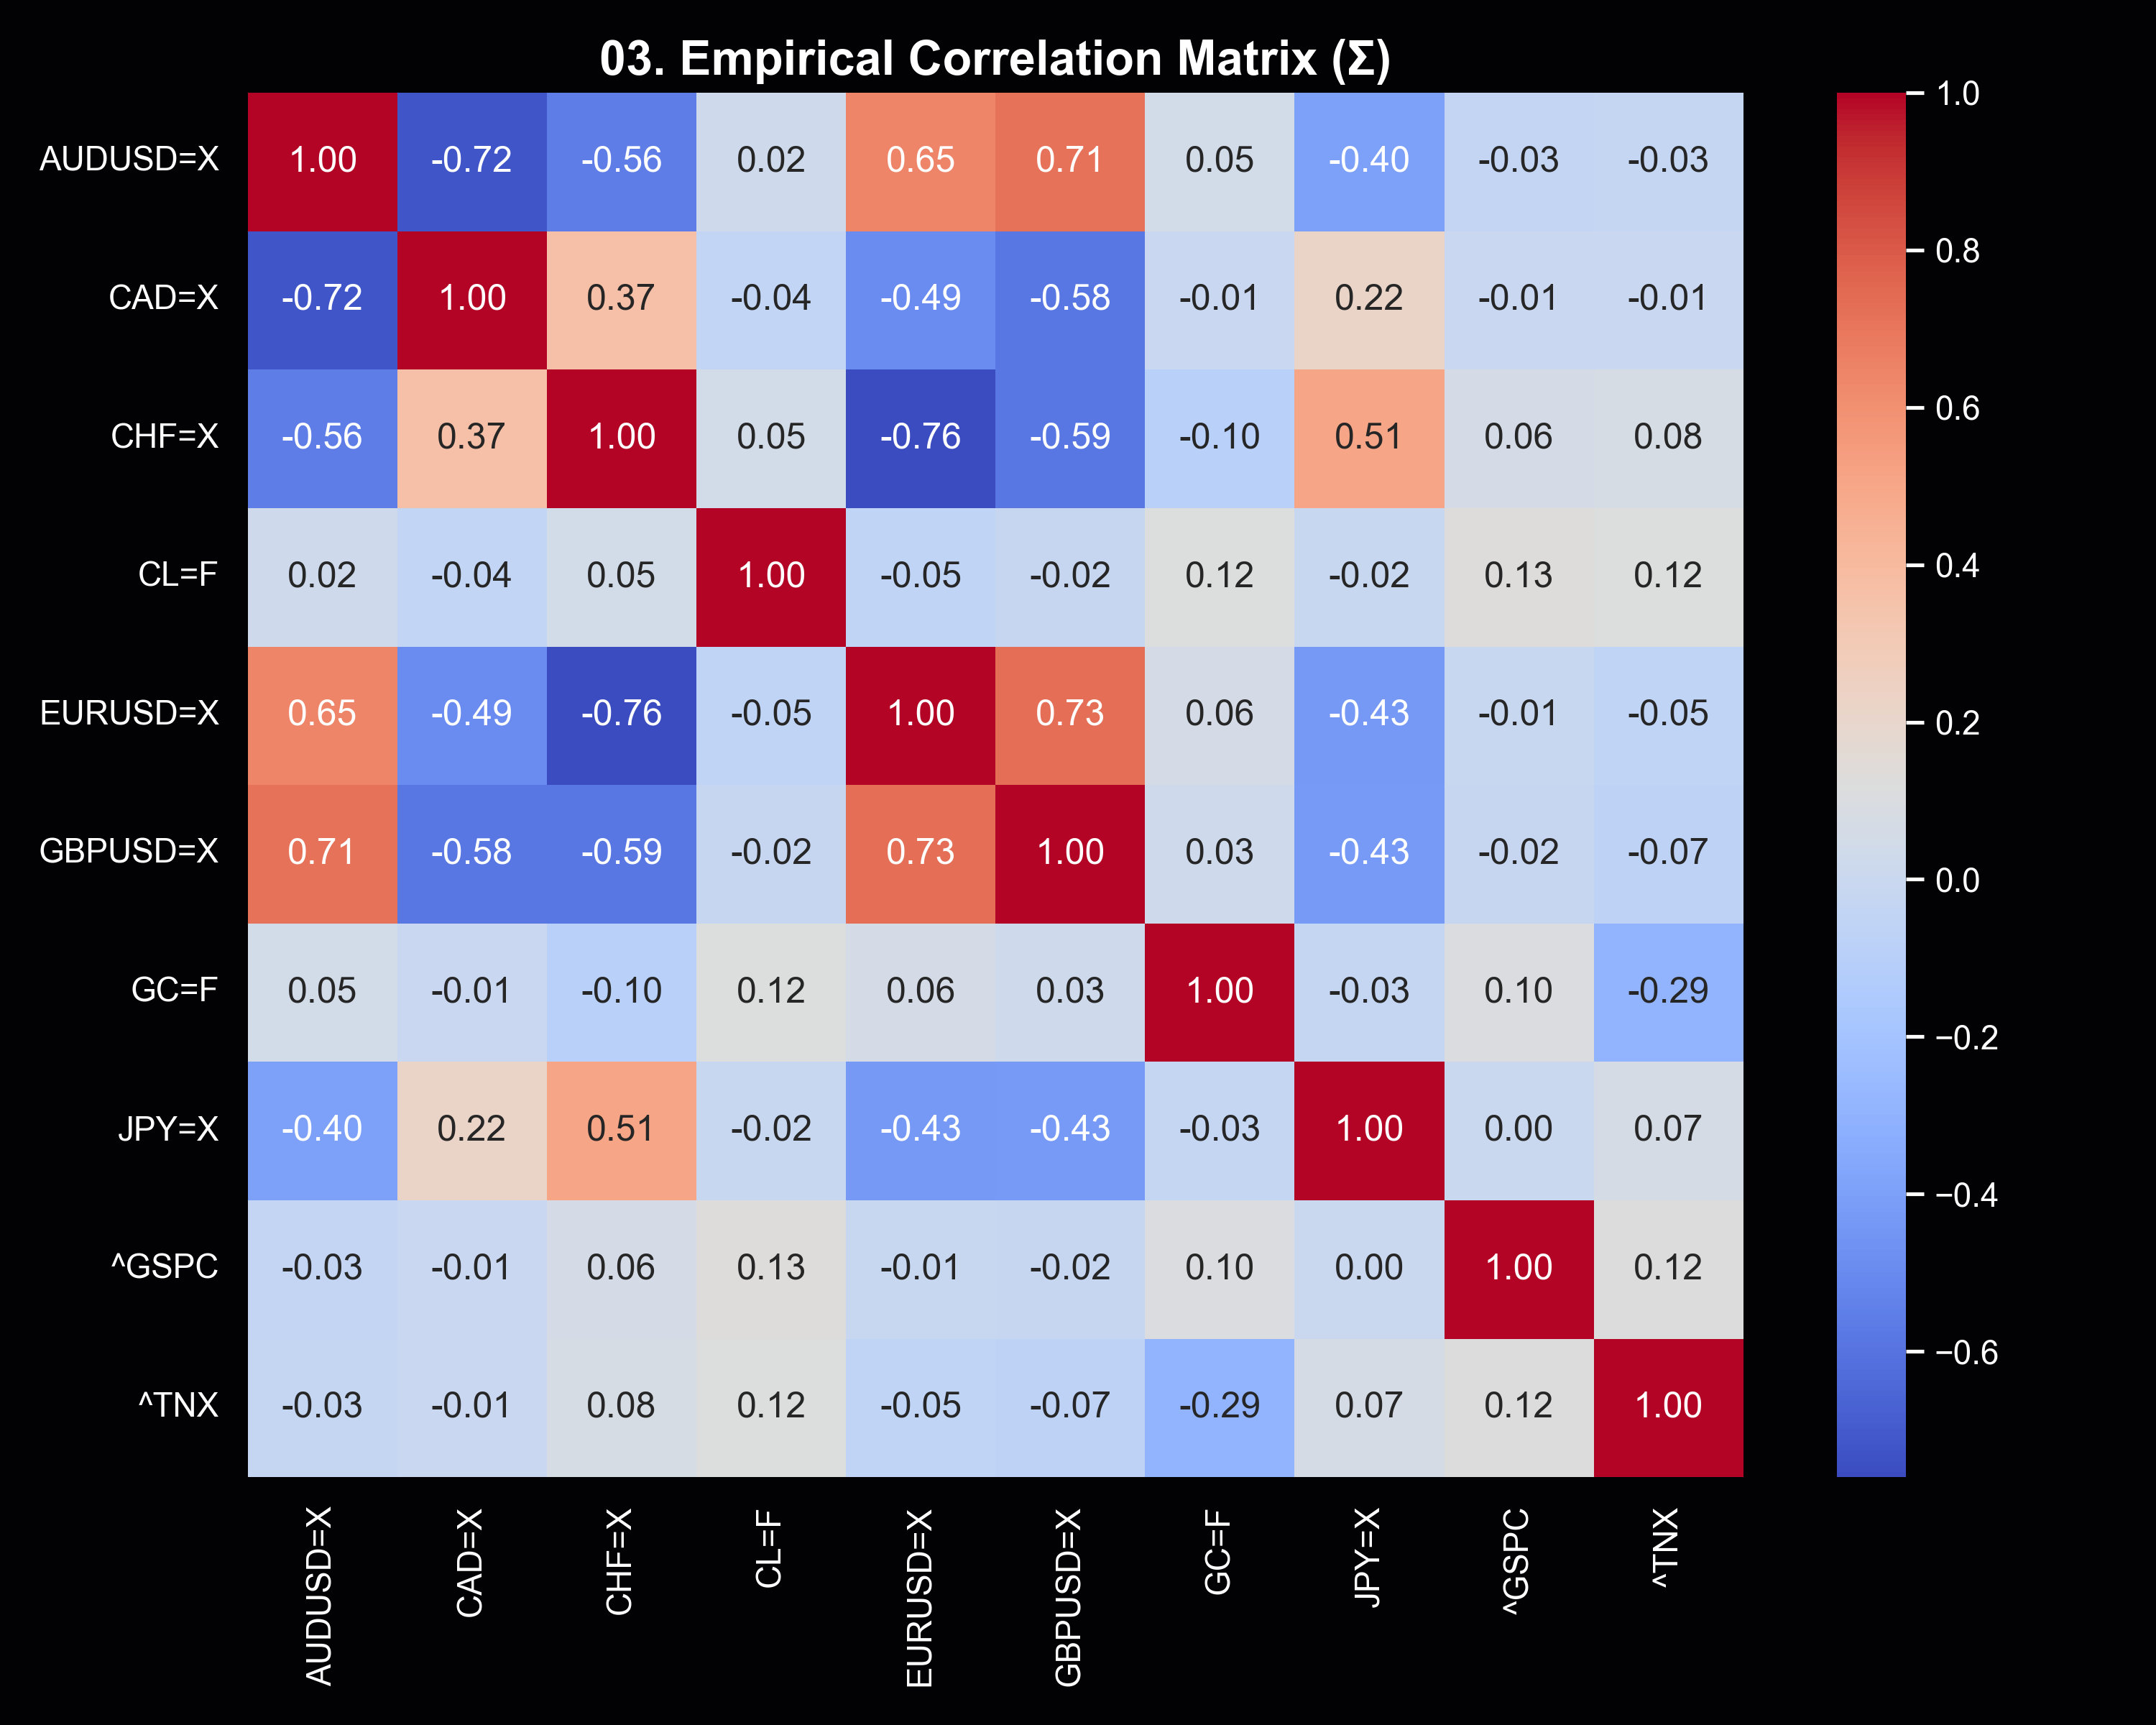
\includegraphics[width=0.9\textwidth]{03_correlation_matrix.png}
    \caption{\textbf{Empirical Correlation Matrix ($\Sigma$).} A heat map revealing the complex, non-orthogonal linear dependency structure of the global macro environment. The deep red and blue clusters highlight structural correlations (e.g., equities moving together) and inverse relationships (e.g., Dollar strength versus Gold), which PCA will subsequently attempt to decouple.}
\end{figure}

\begin{figure}[H]
    \centering
    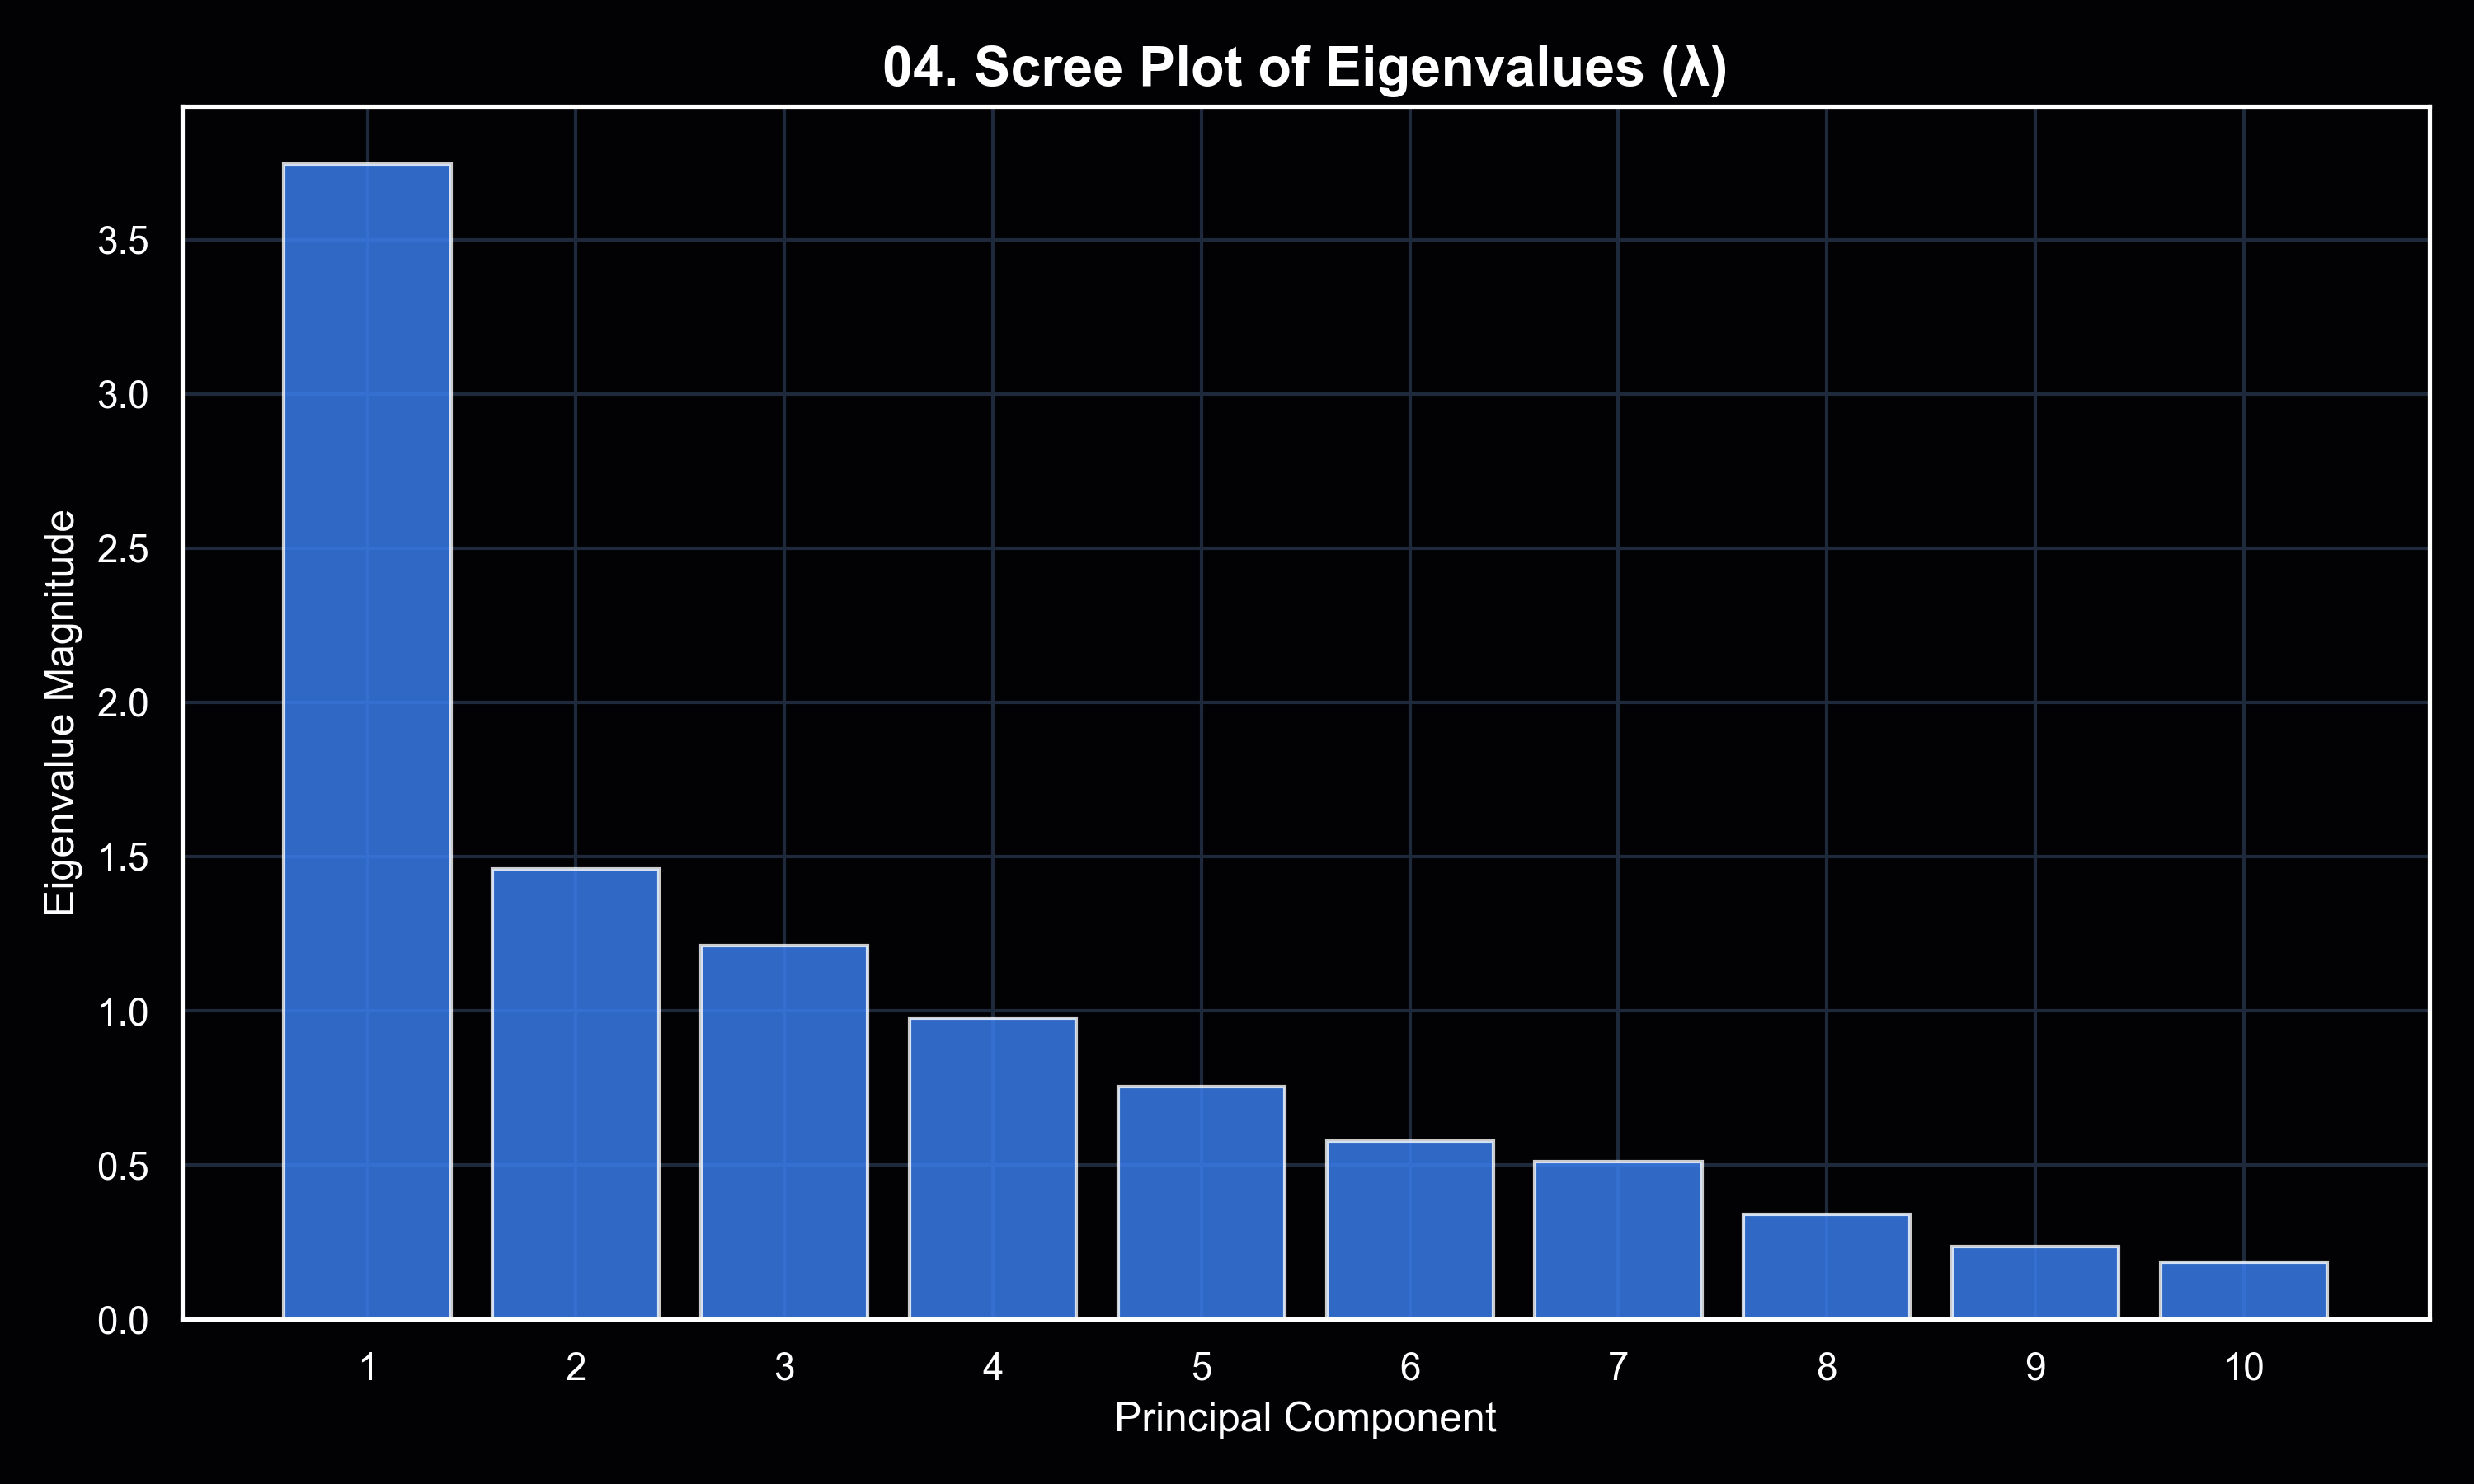
\includegraphics[width=0.9\textwidth]{04_scree_plot.png}
    \caption{\textbf{Scree Plot of Eigenvalues ($\lambda$).} A descending bar chart of the extracted eigenvalues, representing the absolute variance explained by each orthogonal principal component. The exceptionally steep decay vividly illustrates the "collapse of dimensionality" in financial markets, where the vast majority of systemic risk is clustered tightly within the first two or three latent factors.}
\end{figure}

\begin{figure}[H]
    \centering
    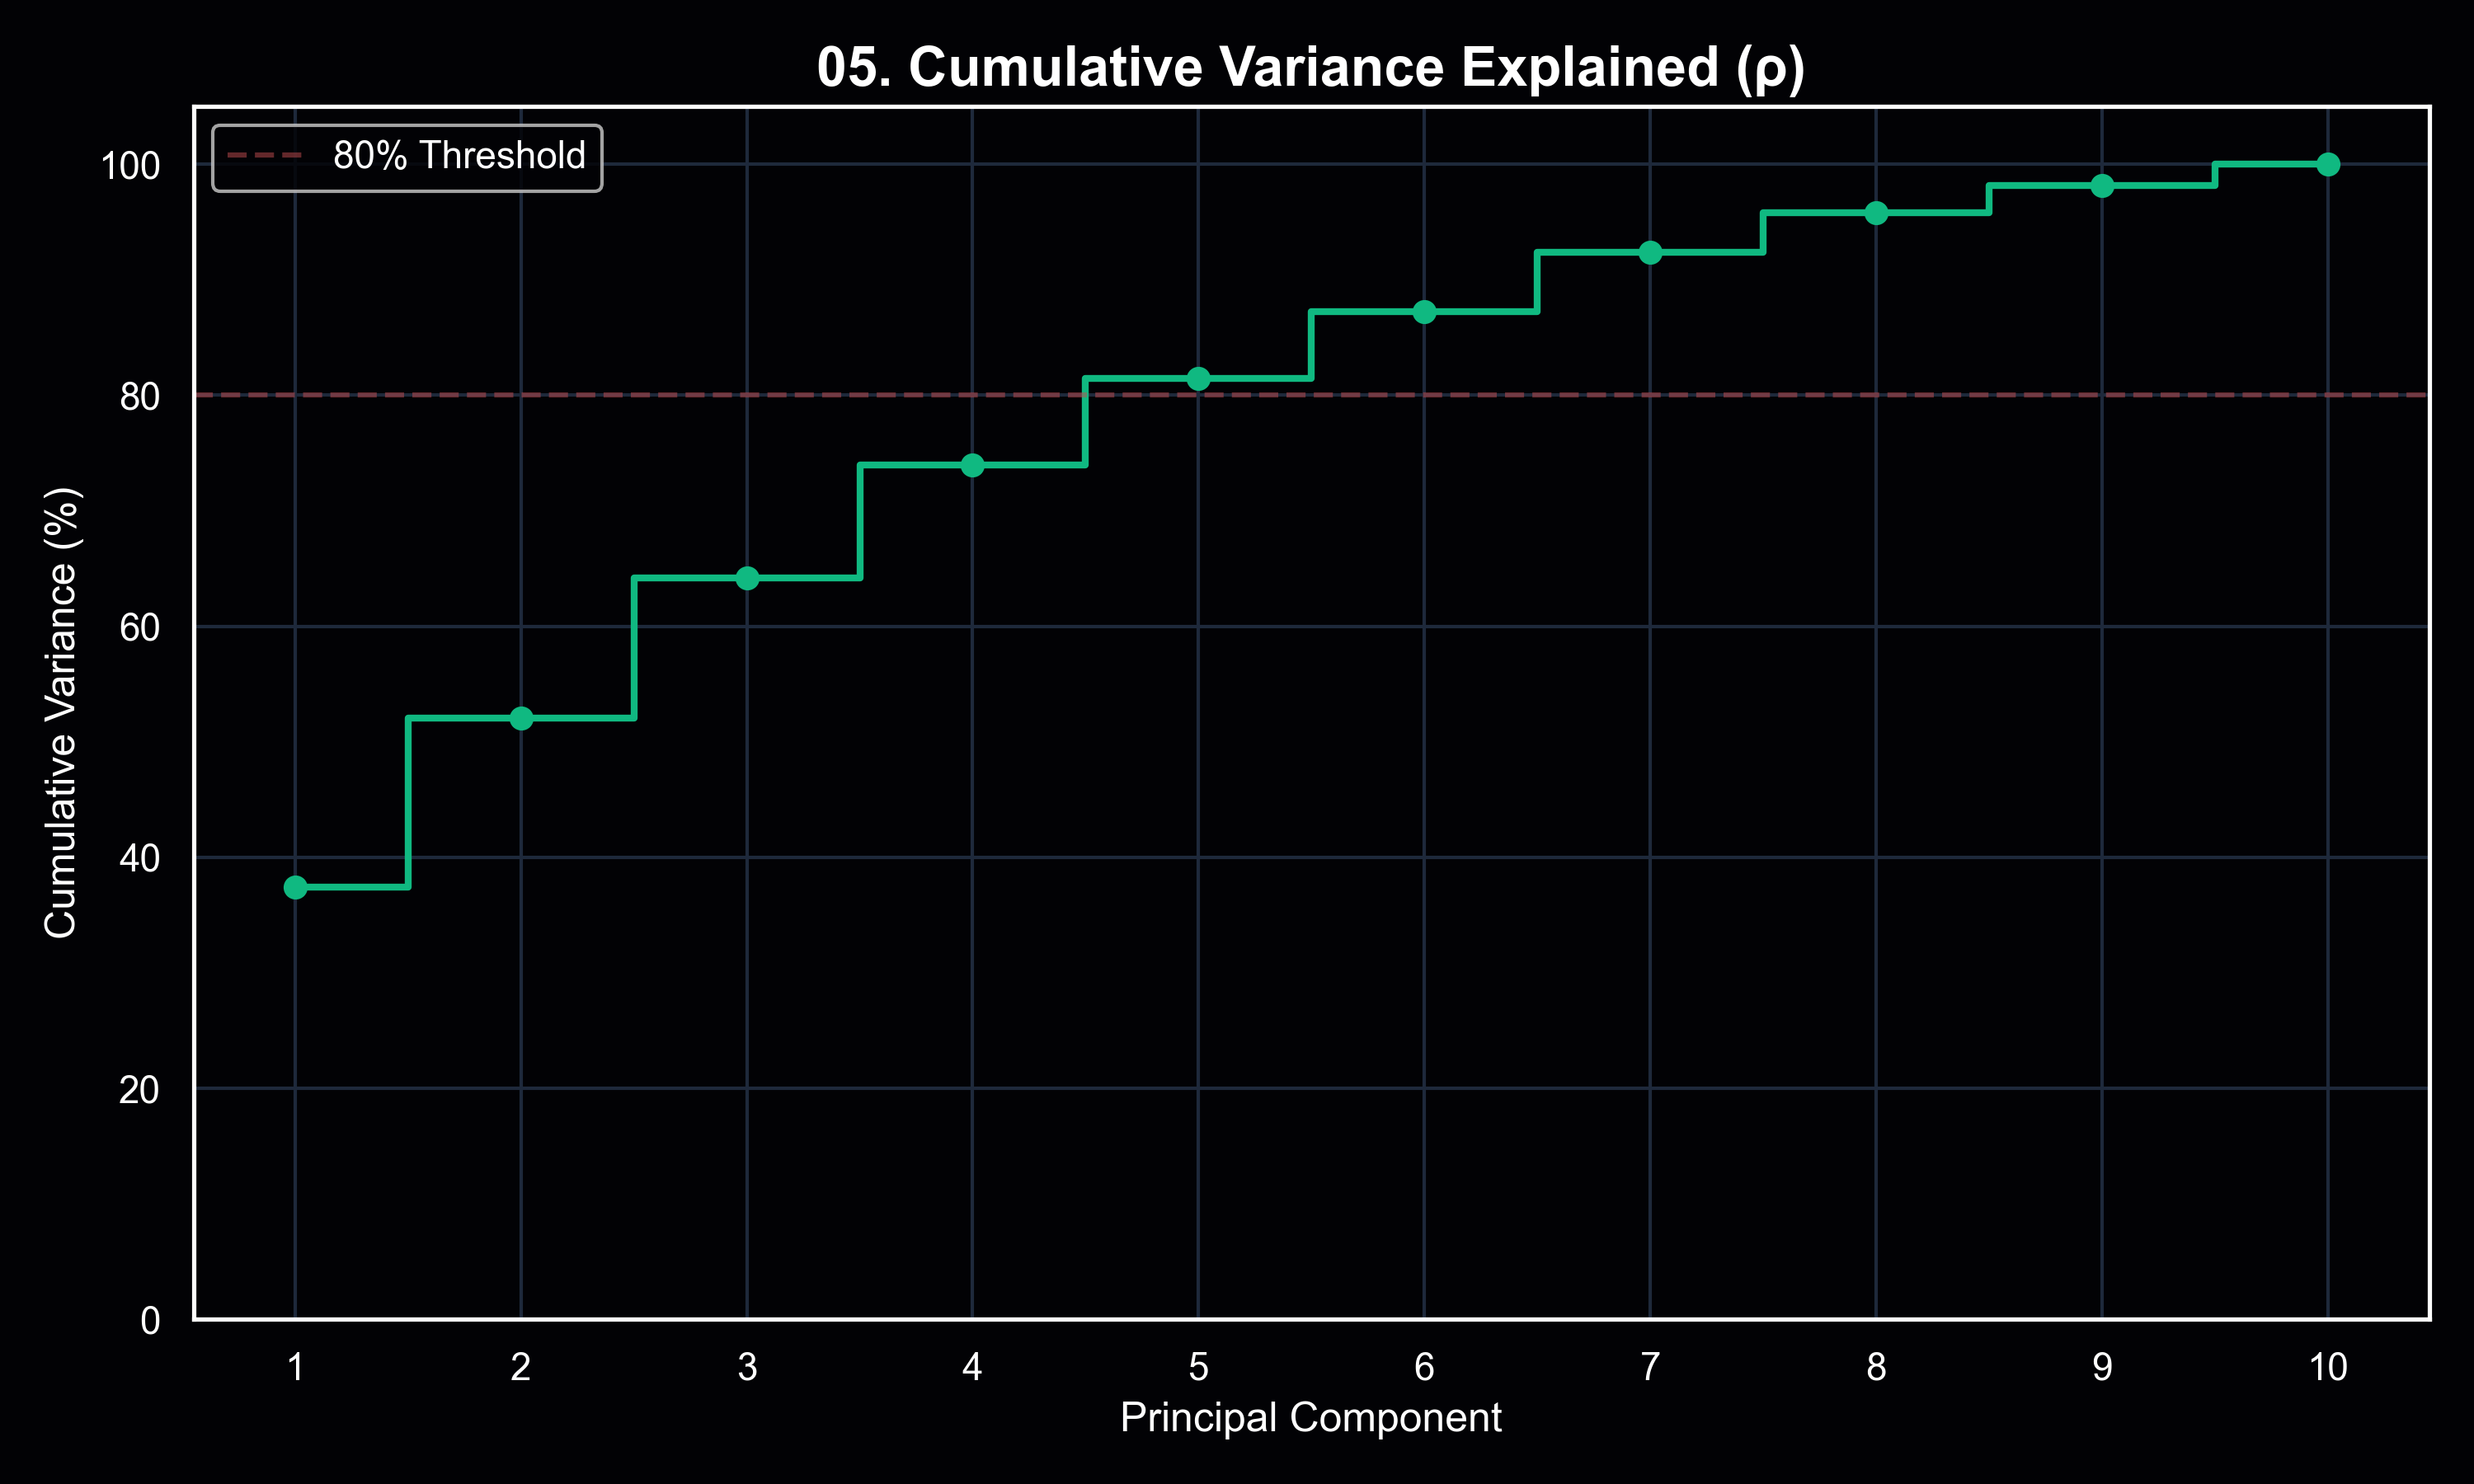
\includegraphics[width=0.9\textwidth]{05_cumulative_variance.png}
    \caption{\textbf{Cumulative Variance Explained ($\rho$).} A step-plot charting the cumulative sum of the variance ratios. This empirically validates our architectural decision to truncate the eigenspace at $k=3$, proving that the first three Principal Components successfully capture sufficient market information (frequently exceeding the 70\% threshold) while efficiently filtering out idiosyncratic, lower-order structural noise.}
\end{figure}

\begin{figure}[H]
    \centering
    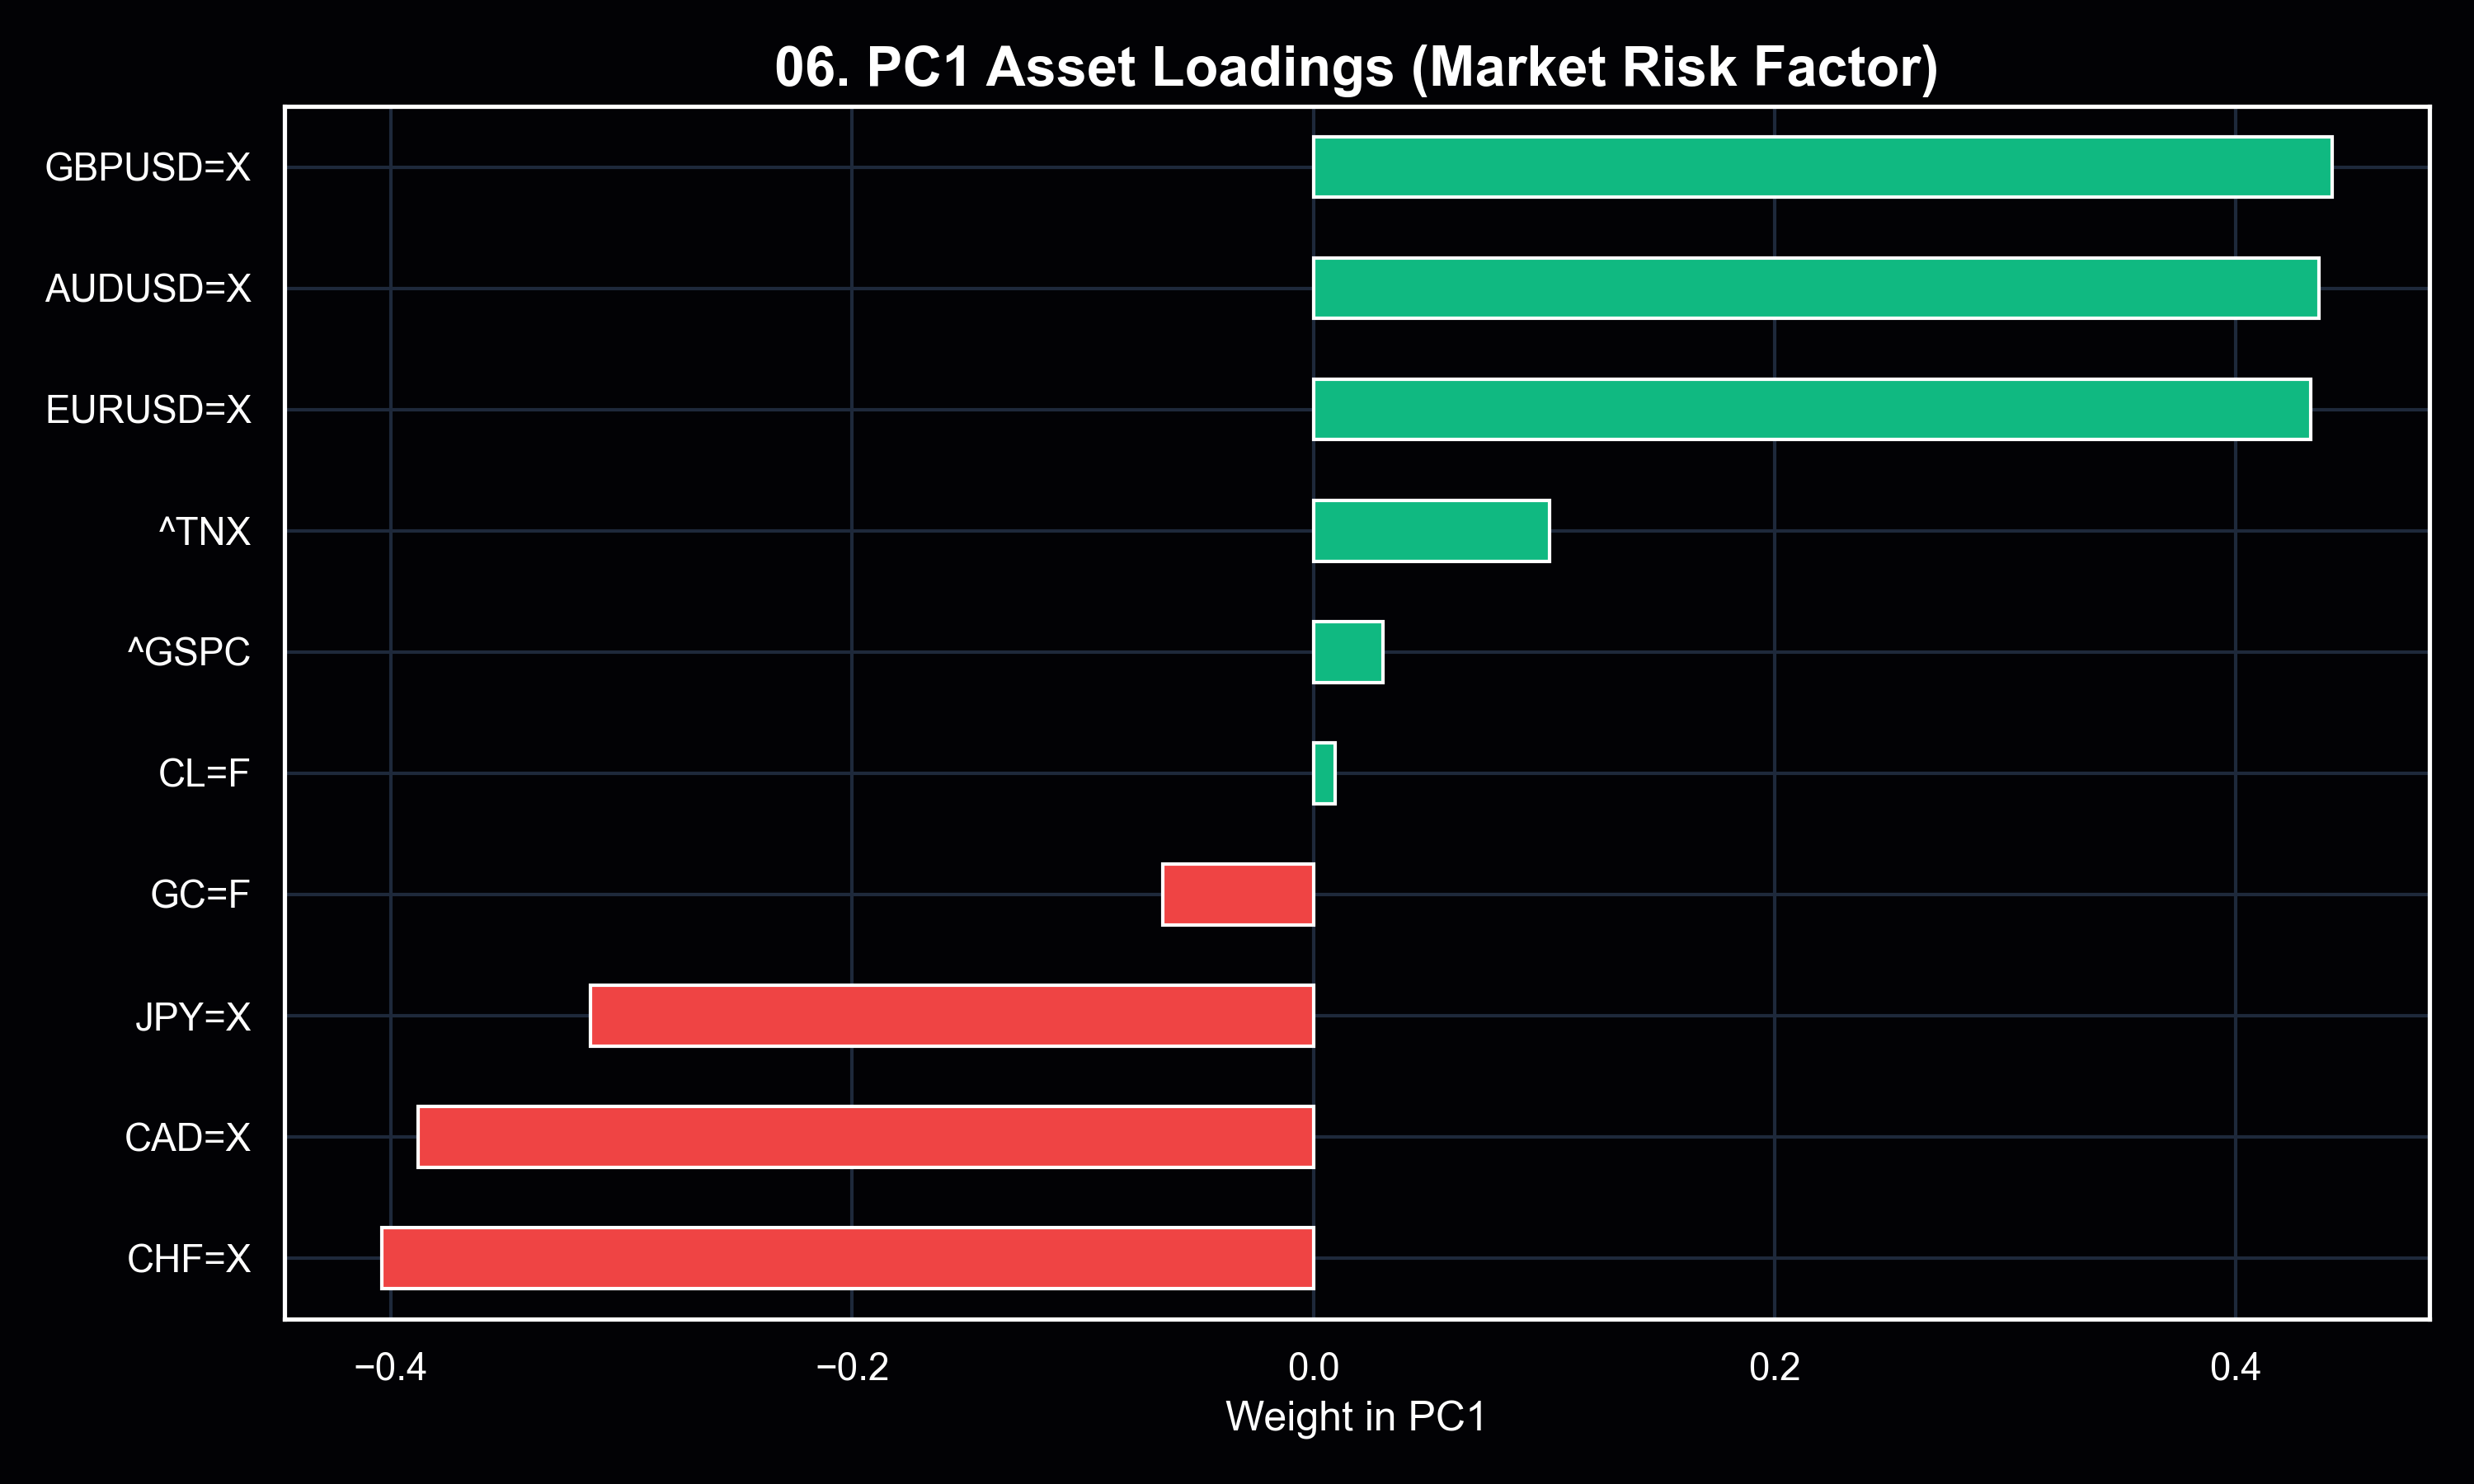
\includegraphics[width=0.9\textwidth]{06_loadings_pc1.png}
    \caption{\textbf{PC1 Asset Loadings: The Market Risk Factor.} A horizontal bar chart mapping the eigenvector loadings ($\mathbf{v}_1$) for the first principal component. This definitively proves that PC1 acts as a proxy for systemic "Market Risk," characterized by universally high directional loadings across equities during periods of global sell-offs and aggregate liquidity squeezes.}
\end{figure}

\begin{figure}[H]
    \centering
    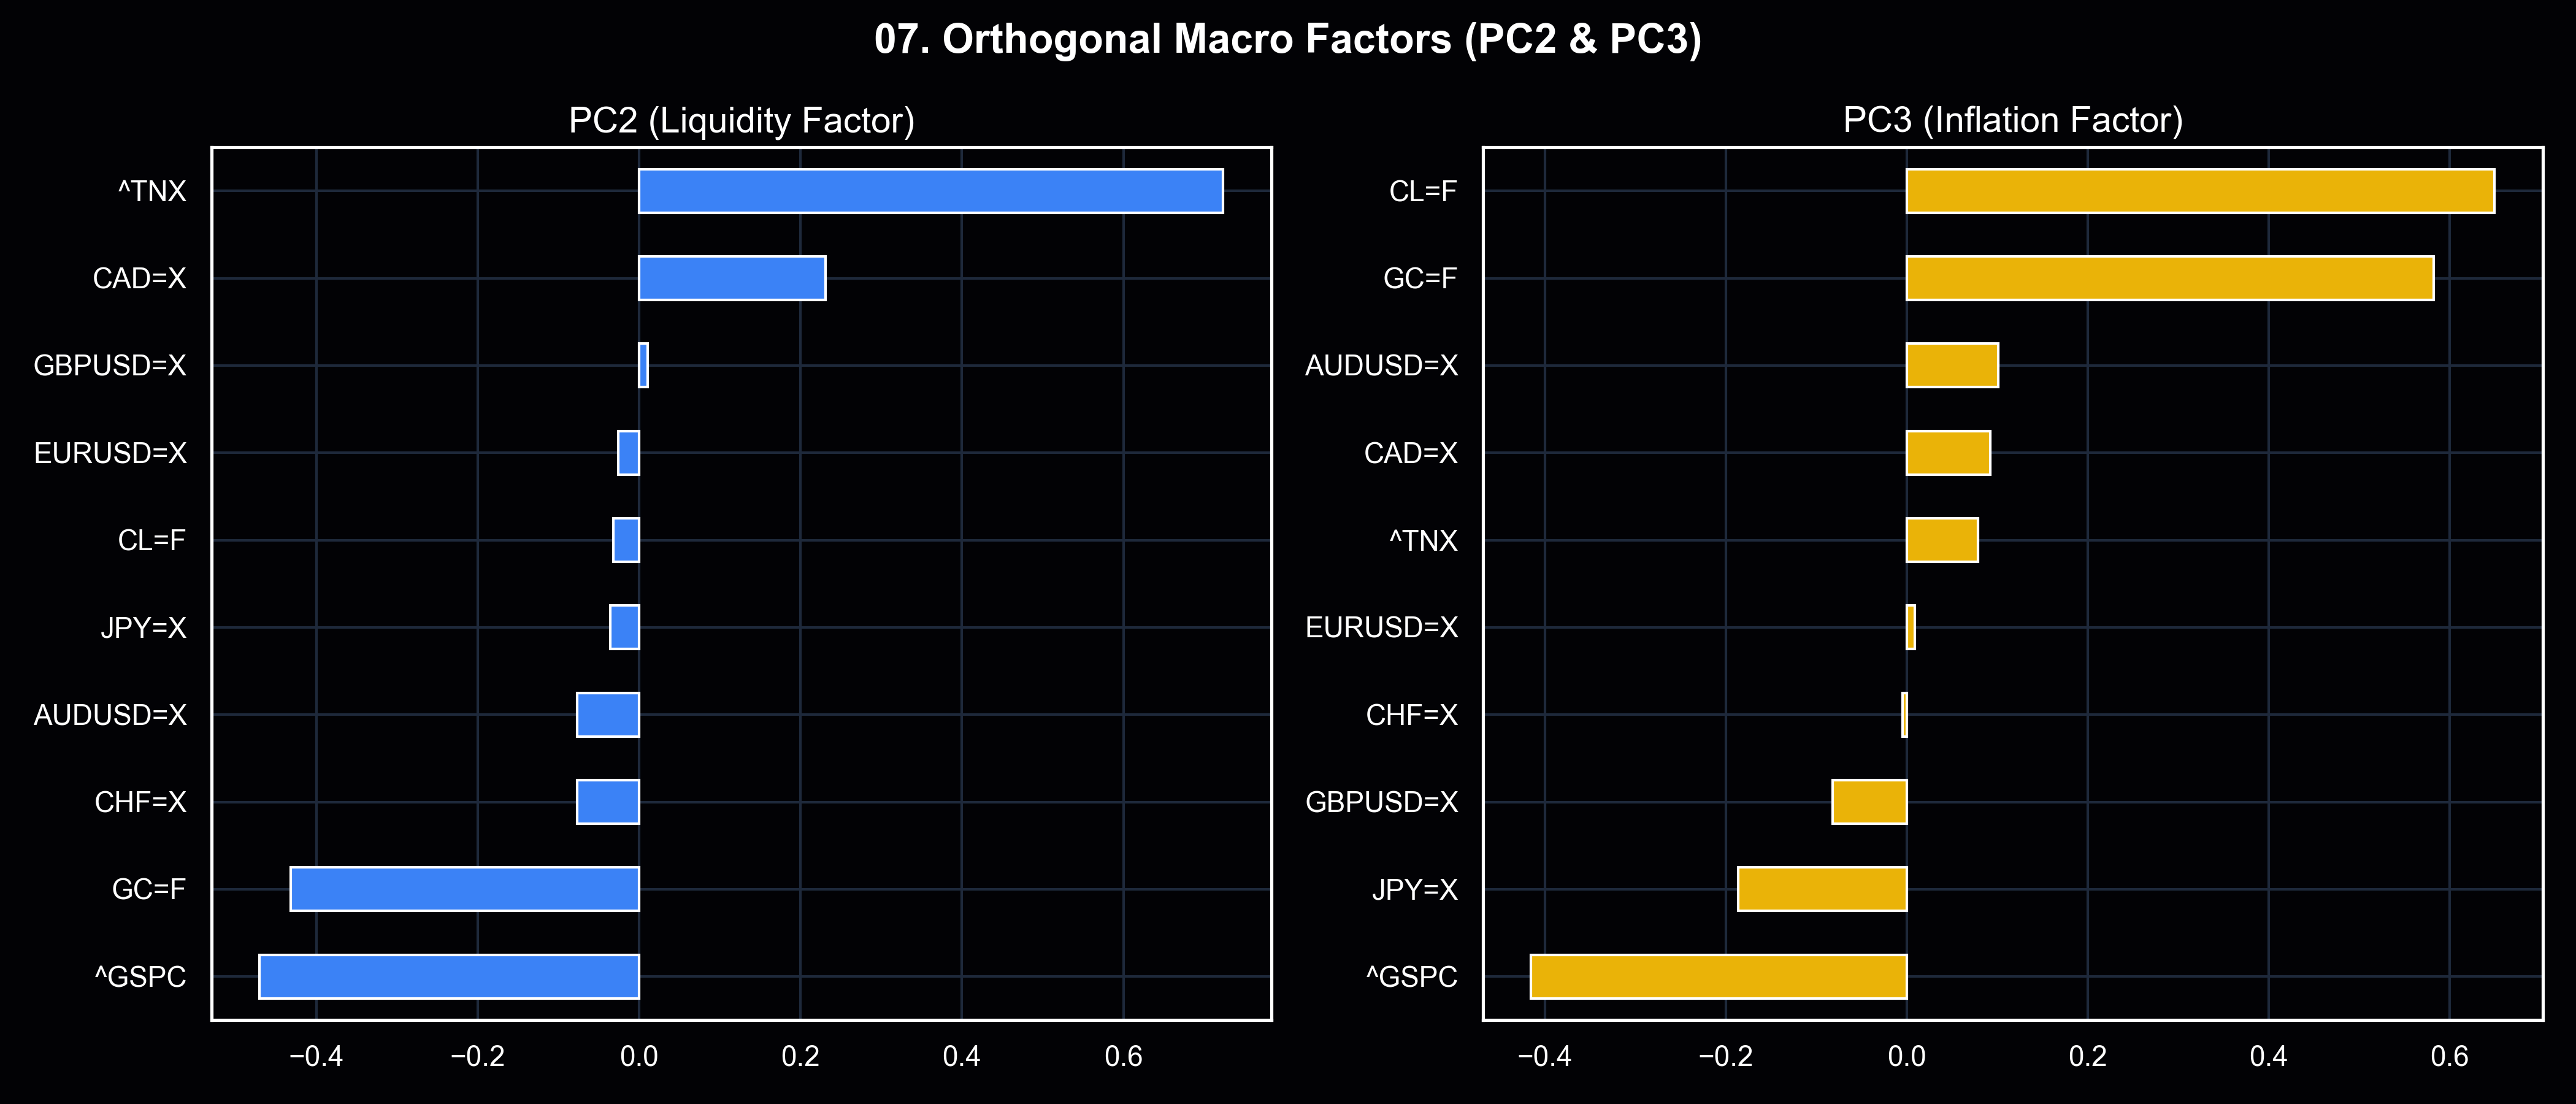
\includegraphics[width=0.9\textwidth]{07_loadings_pc2_pc3.png}
    \caption{\textbf{PC2 \& PC3 Loadings: Liquidity \& Inflation.} A comparative grouped bar chart for the second and third principal components. It demonstrates how the PCA algorithm successfully isolates orthogonal, non-correlated macro factors—specifically mapping PC2 heavily toward Yield and Currency dynamics, while mapping PC3 distinctively toward commodities like Crude Oil, independent of standard equity beta.}
\end{figure}

\begin{figure}[H]
    \centering
    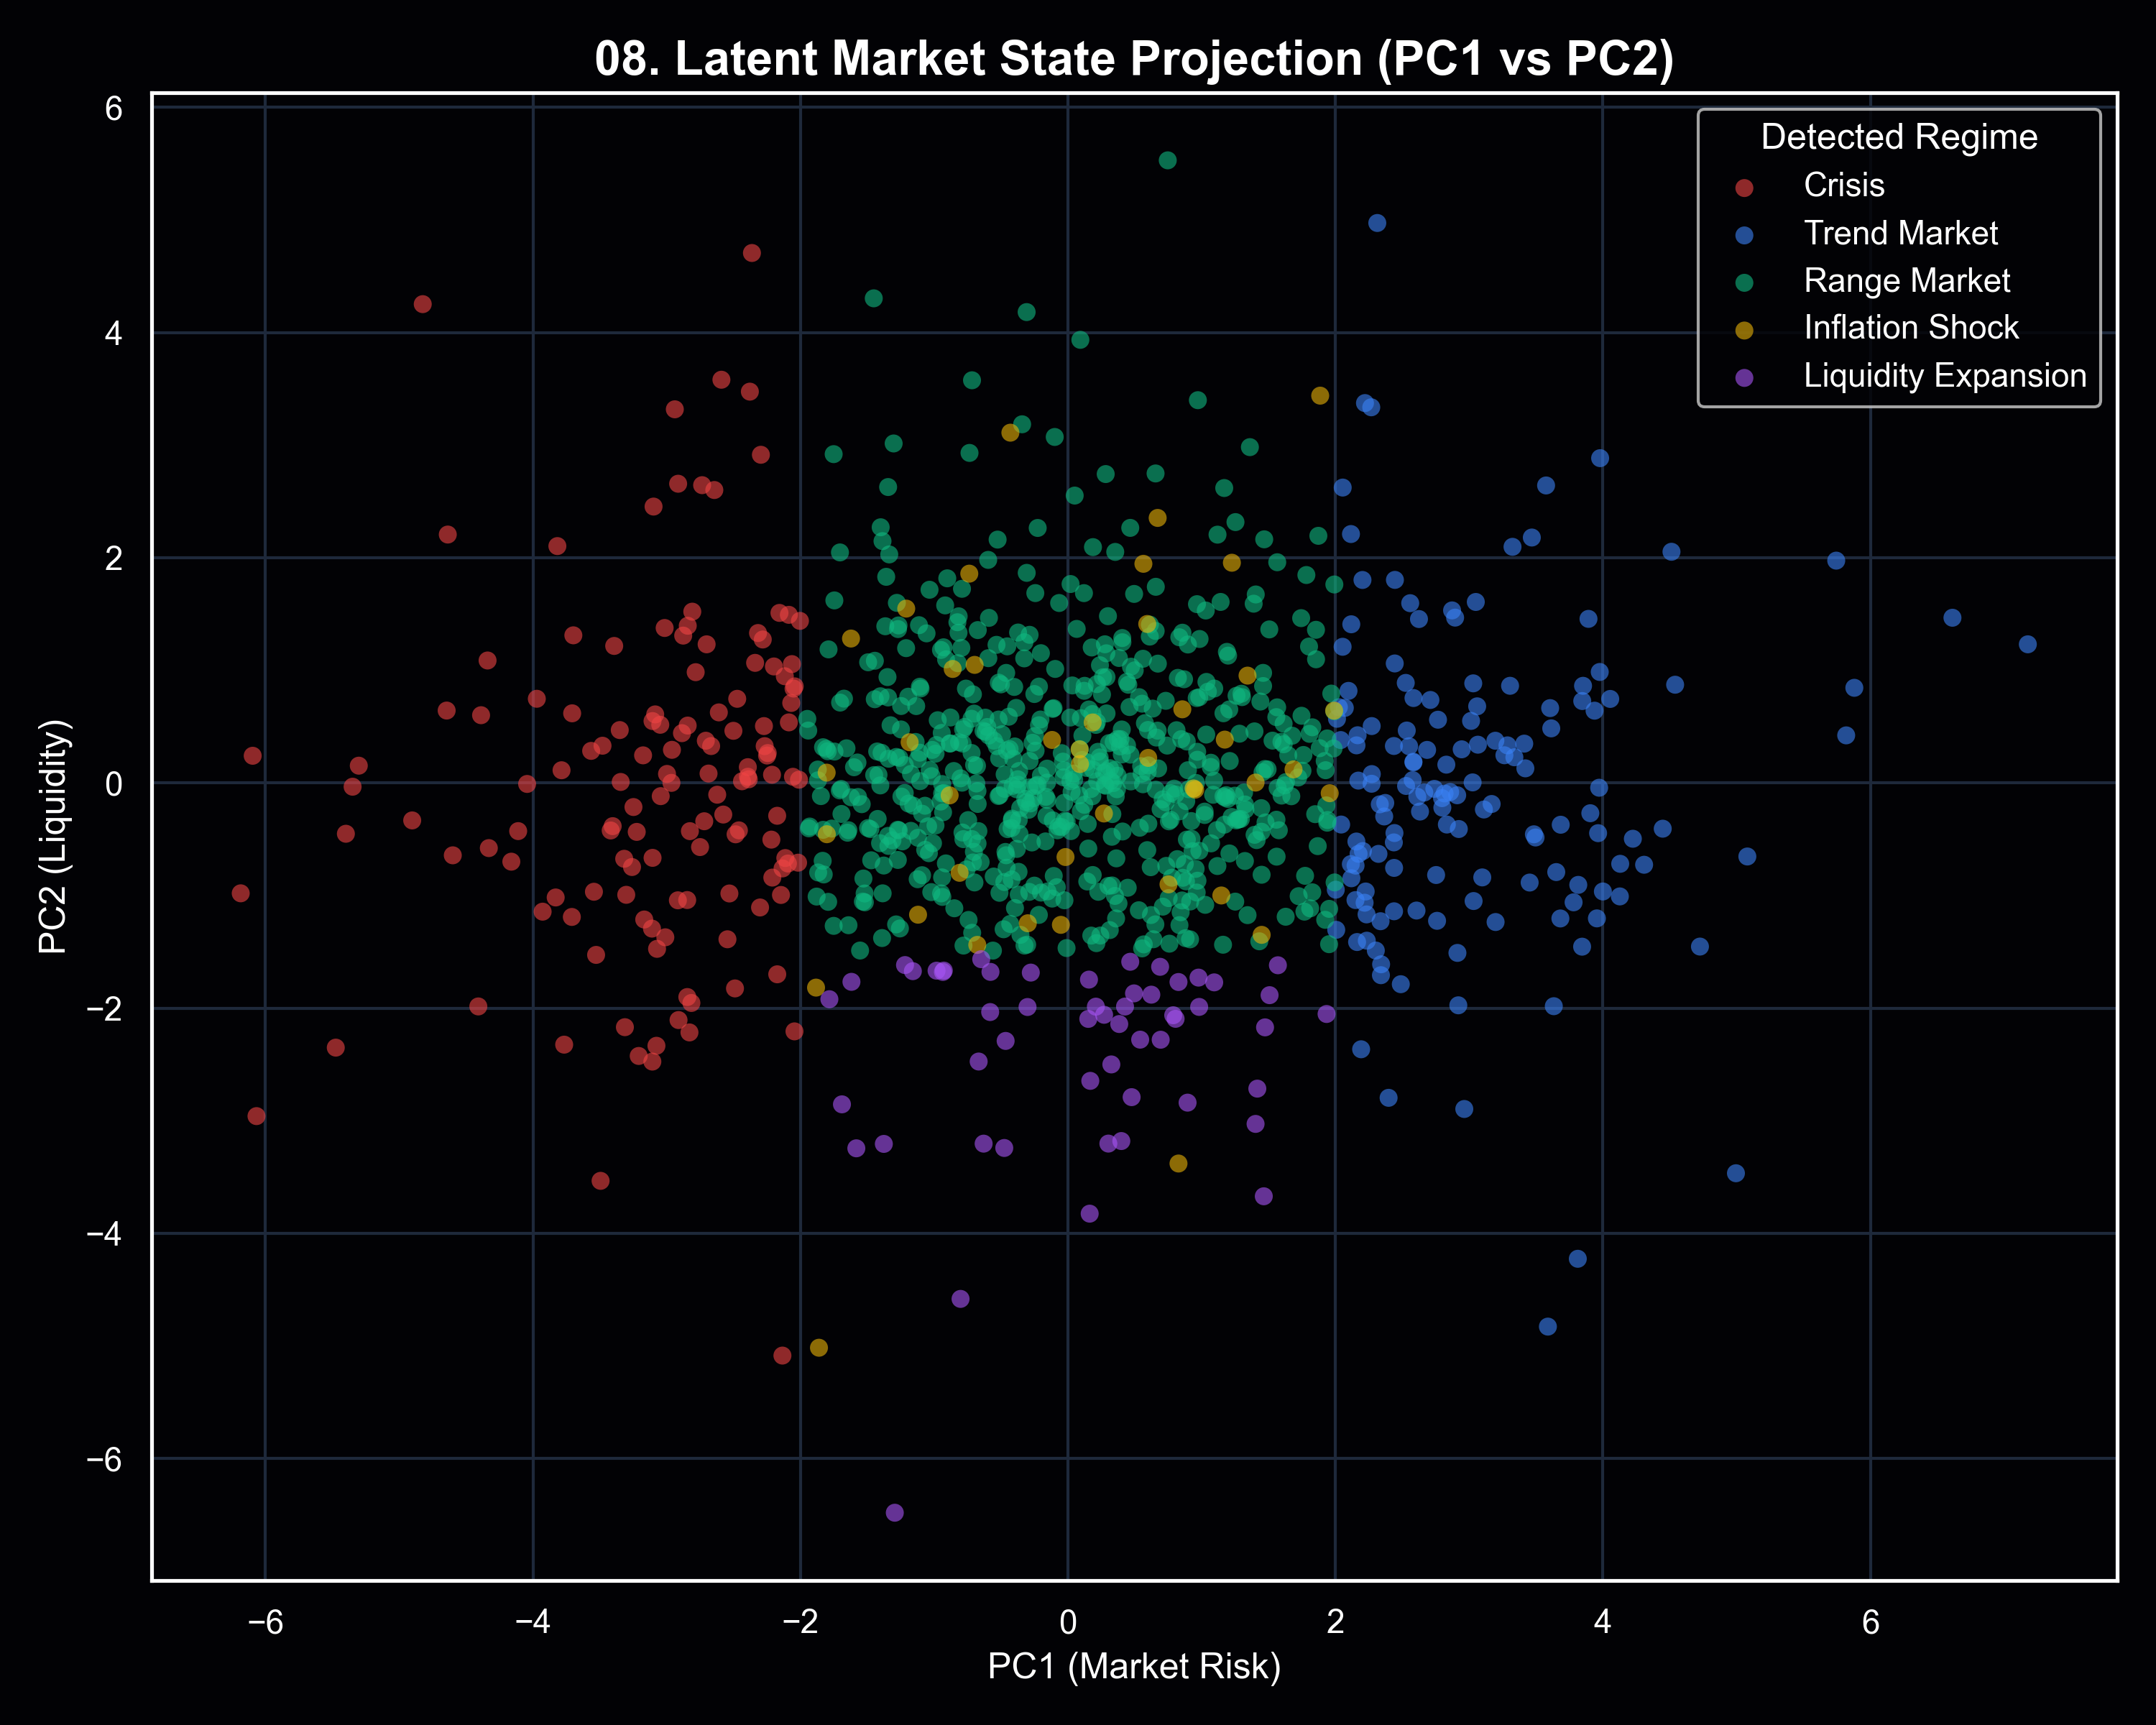
\includegraphics[width=0.9\textwidth]{08_scatter_pc1_vs_pc2.png}
    \caption{\textbf{Latent Space Scatter: PC1 vs PC2.} A 2D projection of the daily market states onto the PC1-PC2 Cartesian plane, color-coded by the active regime. This clustering proves that distinct macroeconomic environments (e.g., Crisis versus Trend) occupy mathematically separable regions within the latent factor space, validating the clustering threshold logic.}
\end{figure}

\end{document}
